%\documentclass[sigconf]{acmart}
\documentclass[sigconf]{llncs}

\usepackage{microtype}
\usepackage{graphicx}
\usepackage{color}
\usepackage{amssymb}
\usepackage{amsmath}
%\setcounter{tocdepth}{3}
\usepackage{graphicx}
\usepackage{tikz}
\usepackage{pgfplots}
\usepackage{framed}
\usepackage{listings}
\usepackage{algorithm,algpseudocode}
\usepackage{epstopdf}
\usepackage{pifont}
\usepackage{todonotes}
\usetikzlibrary{positioning, automata, shapes.arrows, calc, shapes, arrows}
\usetikzlibrary{patterns}
\usepackage{url}

\newcommand{\jrronly}[1]{{}}
\newcommand{\mat}[1]{\boldsymbol{#1}}
\renewcommand{\vec}[1]{\boldsymbol{#1}}
%\newtheorem{theorem}{Theorem}
%\newtheorem{corollary}{Corollary}
%\newtheorem{proof}{Proof}

\newcommand\tool{{\sf DSSynth}}

\begin{document}

\title{Formal Synthesis of Digital Controllers for Observable Continuous
Plants with Transient Performance Specifications}

\author{Dario Cattaruzza, Alessandro Abate, Cristina David, Daniel Kroening}%\email{alessandro.abate@cs.ox.ac.uk}
%\email{dario.cattaruzza@cs.ox.ac.uk}
%\author{Cristina David}\email{cristina.david@cs.ox.ac.uk}
%\email{kroening@cs.ox.ac.uk}


%\end{frontmatter}

\maketitle

%\begin{keyword}                   
%Digital Control; A/D converters; Control System Synthesis; Safety Analysis; Quantization Errors; Observer-based Controller. Sampling.
%\end{keyword}                             

\begin{abstract} 
%
We present a sound and automated approach to synthesizing safe,
digital observer-based controllers for physical plants represented as
linear, time-invariant models.  Models are given as dynamical
equations with inputs, evolving over a continuous state space and
accounting for errors caused by the digitization effects of the
controller.  We use a two-stage counterexample-guided inductive
synthesis (CEGIS) driven by abstraction refinement: (1) The first,
coarse, synthesis stage uses a low resolution discretized model of the
original one and, initially, only looks at static properties of the
system.  (2) The second synthesis stage uses eigendecomposition to
refine the imprecise result computed by the first stage.  Whenever the
second stage is unable to find a candidate solution, it triggers an
abstraction refinement phase, resulting in a finer abstraction being
fed back to the first stage.  This design resulted in a significant
speed-up compared to a traditional single stage one.  We demonstrate
the practical value of this approach by automatically synthesizing
safe observer-based controllers for physical plant models from the
digital control literature.
%
\end{abstract}

\section{Introduction}

Modern implementations of embedded control systems have proliferated with
the availability of low-cost devices that can perform highly non-trivial
control tasks, with significant impact in numerous application areas such as
life sciences, environmental control and robotics~\cite{astrom1997computer,Franklin15}.  Correct synthesis is non-trivial, even in cases with
restricted dynamics.  We examine the case of Linear Time Invariant (LTI)
models, for which the synthesis of controllers is well understood.  However,
the use of digital control architectures adds new challenges caused by
artifacts specific to digital control, such as the effects of
finite-precision arithmetic, time discretization and quantization errors
introduced by A/D and D/A conversion.

While research on digital control is well
developed~\cite{astrom1997computer}, automated and sound control synthesis
is challenging, particularly when the synthesis objective goes beyond
classical stability.  Recent work~\cite{abate2017automated} described a
method for synthesising safe digital stabilizing controllers for fully
observable LTI plants.  This work differs from the vast majority of existing
approaches in that it explores the continuous space of the system to
synthesise correct by construction minimal digital controllers.  Contrary to
LTL models \todo{citation} that require thousands of states and elaborate algorithms to
implement, these PID-like controllers are represented by a few parameters
and only require a few lines of code, thus reducing the implementation cost
and execution time while remaining resilient to the effects of digitalization.
However,~\cite{abate2017automated}~is restricted to fully observed
systems (i.e., where all the states are known) modelled in discrete time,
and furthemore explores only a limited set of properties that engineers
are interested in. Conversely, 
in most real implementations, the internal state of a plant cannot be
directly measured but rather inferred from its
effect on the output. A plant model that minimises the difference
between the outputs is called an observer and it is a well known
paradigm in the control literature~\cite{astrom1997computer}.


In this paper we build on the ideas presented in~\cite{abate2017automated}
and develop a new technique that addresses most of these limitations. 
By~combining state-of-the-art synthesis and verification engines we
automatically generate digital observer controllers for a given continuous
plant model that are correct by construction.  %% This approach delivers a high
%% degree of automation, promises to reduce the cost and time of development of
%% digital control dramatically, and requires considerably less expertise than
%% a-posteriori verification.
Specifically, we synthesize stable,
software-implemented embedded controllers along with a model of a physical
plant (observer).  Due to the complexity of such closed-loop systems, in
this work we focus on linear models with known configurations, and perform
parametric synthesis of controllers meeting a number of properties that
define their desired behaviour.

We perform digital control synthesis over a hybrid model, where the plant
exhibits continuous behavior whereas the controller operates in discrete
time and over a quantized domain.  Our model evaluates the effects of the
quantizers (A/D and D/A converters) and of time discretization, as well as
representation errors introduced by modelling artifacts such as an
observer~\cite{astrom1997computer} in a finite precision domain, while
reasoning about high level properties such as stability, robustness, safety,
and response time, which define the behaviour of the system.  In particular,
safety requirements are frequently overlooked in conventional feedback
control synthesis, but play an important role in systems engineering.

%% Using state of the art verifiers, we evaluate these models against
%% automatically synthesised controllers using CEGIS-based synsthesis that
%% incorporate the above mentioned artifacts in different models of
%% Single-Input/Single-Output (SISO) systems.  We offer a multi-tiered approach
%% that exploits different aspects of the problem at each stage.

We make use of a two-stage counterexample-guided inductive
synthesis (CEGIS) driven by abstraction refinement.
The first, coarse, synthesis stage uses a low resolution discretized model of a 
transformation of the original model. Furthermore, it only looks initially at
static properties  of the system. This largely reduces the complexity of
the problem, enabling the synthesiser to offer fast response times. %% If any 
%% of these parameters is inadequate, the refinement loop will supply a better
%% abstraction to obtain a feasible answer.
Due to either numerical imprecision or overapproximations, the
candidate solution presented by the first synthesiser will likely not
meet the spec. A second synthesis stage, with a much more precise
refinement including a mapping between the real and transformed spaces
will create a candidate solution that is more adequate to the real
model. This second stage uses perturbation analysis and therefore
requires an initial solution to operate.  Whenever the second stage is
unable to find a candidate solution, it triggers an abstraction
refinement phase, resulting in a finer abstraction being fed back to
the first stage.  The combined synthesisers are thus capable of
reasoning about complex models with high computational efficiency due
to their modularity.

%The synthesiser uses a discrete time model that relates to the sampling
%time.  It begins with a very simple abstraction of the real system which
%only considers the static properties of the model.  It~also uses a very low
%precision bit vector representation of the real dynamics in order to
%minimise synthesis time.  
%% A candidate solution is then passed to a set of verifiers which will
%% evaluate the synthesised controller over an even more precise
%% abstraction of the concrete domain in both discrete and continuous
%% space/time.  The verification phase uses abstraction refinement when needed to ensure
%% that rejected candidates are not being discarded due to the
%% over-approximation.

%% The nature of the counterexamples varies depending on
%% the following conditions:
%% %
%% \begin{enumerate}
%% %
%% \item Initially, we look for possible errors caused by the restricted domain
%% of the synthesisers (e.g., overflows and rounding).  These will typically 
%% manifest in the static properties of the system. If an error is found, the
%% modeller is signalled to increase the precision of the synthesisers.
%% %
%% \item Next we explore the nature of the discrete-time progression to mark
%% a counterexample that relates to the progression of the system. If such a
%% counterexample exists, we indicate its initial conditions and time horizon,
%% thus instructing the synthesiser to refine its abstraction with respect to the
%% set of initial states and number of iterations. 
%% %
%% \item Continuous time analysis indicates the need for decreasing the
%% sampling time due to continuous excursions outside the safety region in
%% between samples.  This changes the problem statement of the synthesiser to a
%% new discrete-time model.
%% %
%% \item A final condition arises when a candidate solution cannot be found,
%% thus requiring higher precision of the abstraction numerical representation. 
%% We initially consider the plant representation to be too conservative and
%% may eventually increase the controller FWL specification when no controller
%% can be found for a given precision.
%% %
%% \end{enumerate}

We provide experimental results showing that our approach is able to
efficiently synthesize safe controllers for a set of physical
plant models taken from the digital control literature.

In summary, this paper makes the following original contributions.
%
\begin{enumerate}

\item We automatically generate \emph{correct-by-construction} digital
  state-feedback observer controllers that guarantee a given safety property
  alongside stability and response time specifications.  We note that
  observers are much more complex and difficult to synthesise than standard
  full-state feedback controllers.
%
\item  Our synthesis addresses challenges created by digitalization errors
 such as quantization, and time discretization as well as delays in the
 sampling and processing times which introduce control errors in real
 implementations.
 \item we present a model for soundly evaluating reachability in a combined 
 continuous-discrete time/space. Sound tools for continuous time reachability 
 are scarce and to the authors' knowledge no tool provides a model that 
 combines both. 
%
\item We develop a model for inductive synthesis that combines CEGIS with
abstraction refinement in order to minimize the synthesis cost. In particular
we explore the idea of a multi-tiered model where different verification, 
synthesis and modelling tools/modules explore different parts of the problem
to deliver an optimal response.
%
\end{enumerate}

%-------------------------------
\section{Related Work}
\label{sec:relw}
%-------------------------------

\textbf{CEGIS --}
Program synthesis is the problem of computing correct-by-design programs
from high-level specifications.  Algorithms for this problem have made
substantial progress in recent years, for instance~\cite{itzhaky2010simple}
to inductively synthesize invariants for the generation of desired programs.

Program synthesizers are an ideal fit for the synthesis of digital
controllers, since the semantics of programs capture the effects of
finite-precision arithmetic precisely. 
In~\cite{DBLP:conf/cdc/RavanbakhshS15}, the authors use CEGIS for the
synthesis of switching controllers for stabilizing continuous-time plants
with polynomial dynamics.  The work extends to affine systems, but is
limited by the capacity of the state-of-the-art SMT solvers for solving
linear arithmetic.  Since this approach uses switching models instead of
linear dynamics for the digital controller, it avoids problems related to
finite precision arithmetic, but potentially suffers from state-space
explosion.  Moreover, in \cite{DBLP:conf/emsoft/RavanbakhshS16} the same
authors use a CEGIS-based approach for synthesizing continuous-time
switching controllers that guarantee \emph{reach-while-stay} properties of
closed-loop systems, i.e., properties that specify a set of goal states and
safe states (constrained reachability).  This solution is based on
synthesizing control Lyapunov functions for switched systems that yield
switching controllers with a guaranteed minimum dwell time in each mode. 
However, both approaches are unsuitable for the kind of control we seek to
synthesize.

The work in~\cite{hscc-paper} synthesizes stabilizing controllers for
continuous plants given as transfer functions by exploiting bit-accurate
verification of software-implemented digital controllers~\cite{Bessa16}. 
While this work also uses CEGIS, the approach is restricted to digital
controllers for stable closed-loop systems given as transfer function
models: this results in a static check on their coefficients.  By contrast,
in the current paper we consider a state-space representation of the
physical system, which requires ensuring the specification over actual
traces of the model, alongside the numerical soundness required by the
effects of discretisation and finite-precision errors.  A state-space model
has known advantages over the transfer function
representation~\cite{Franklin15}: it naturally generalizes to multivariate
systems (i.e., with multiple inputs and outputs); and it allows synthesis of
control systems with guarantees on the internal dynamics, e.g., to
synthesize controllers that make the closed-loop system \emph{safe}.  Our
work focuses on the \emph{safety} of internal states, which is usually
overlooked in the literature.  Moreover, our work integrates an
abstraction/refinement (CEGAR) step inside the main CEGIS loop.

The tool Pessoa~\cite{mazo2010pessoa} synthesizes correct-by-design embedded
control software in a Matlab toolbox.  It is based on the abstraction of a
physical system to an equivalent finite-state machine and on the
verification of reachability properties on it.  Based on this safety
specification, \mbox{Pessoa} can synthesize embedded controller software for
a range of properties.  The embedded controller software can be more
complicated than the state-feedback control we synthesize, and the
properties available cover more detail.  However, relying on state-space
discretization \mbox{Pessoa} is likely to incur in scalability limitations. 
Along this research line, \cite{Anta2010,liu16} studies the synthesis of
digital controllers for continuous dynamics, and \cite{zamani2014} extends
the approach to the recent setup of Network Control Systems.

\textbf{Discretization Effects --}
The classical approach to control synthesis has often disregarded
digitalization effects, whereas more recently modern techniques have focused
on different aspects of discretization, including delayed
response~\cite{Duggirala2015} and finite word length (FWL) semantics, with
the goal either to verify (e.g.,~\cite{daes20161}) or to optimize
(e.g.,~\cite{oudjida2014design}) given implementations.

There are two different problems that arise from FWL semantics.  The first
is the error in the dynamics caused by the inability to represent the exact
state of the physical system, while the second relates to rounding and
saturation errors during computation.  In~\cite{fialho1994stability}, a
stability measure based on the error of the digital dynamics ensures that
the deviation introduced by FWL does not make the digital system unstable. 
A~more recent approach~\cite{DBLP:journals/automatica/WuLCC09} uses
$\mu$-calculus to directly model the digital controller so that the selected
parameters are stable by design.  The analyses
in~\cite{DBLP:conf/hybrid/RouxJG15,DBLP:conf/hybrid/WangGRJF16} rely on an
invariant computation on the discrete system dynamics using Semi-Definite
Programming (SDP).  While the former uses bounded-input and bounded-output
(BIBO) properties to determine stability, the latter uses Lyapunov-based
quadratic invariants.  In both cases, the SDP solver uses floating-point
arithmetic and soundness is checked by bounding the error.  An alternative
is~\cite{park2016scalable}, where the verification of given control code is
performed against a known model by extracting an LTI model of the code by
symbolic execution: to account for rounding errors, an upper bound is
introduced in the verification phase.  The work in
\cite{picasso2003stabilization} introduces invariant sets as a mechanism to
bound the quantization error effect on stabilization as an invariant set
that always converges toward the controllable set.  Similarly,
\cite{liberzon2003hybrid} evaluates the quantization error dynamics and
bounds its trajectory to a known region over a finite time period.  This
technique works for both linear and non-linear systems.

%-------------------------------
\section{Preliminaries}
\label{sec:preliminaries}
%-------------------------------

%+++++++++++++++++++++++++++++++++++++++++++++++++++++++++++++++++++++++++++++++
\subsection{Model Semantics}\label{sec:model_semantics}
%+++++++++++++++++++++++++++++++++++++++++++++++++++++++++++++++++++++++++++++++

\todo{This section should be integrated later, closer to the use of AA}

The traces of the model starting from an initial set $X_0\subseteq \mathbb{R}^p$, 
with inputs restricted to $U \subseteq \mathbb{R}^q$, are sequences 
$ \vec{x}_0 \xrightarrow{\vec{u}_0} \vec{x}_1 \xrightarrow{\vec{u}_1} \vec{x}_2 \xrightarrow{\vec{u}_2} \ldots $, 
%
where $ \vec{x}_0 \in X_0$ and $\forall k\geq 0, \vec{u}_k \in U \text{ and } \vec{x}_{k+1} = \tau(\vec{x}_k,\vec{u}_k) $, 
where 
%
\begin{equation}\label{equ:reachtraj}
\tau(\vec{x}_k,\vec{u}_k) = 
\big( \mat{A}\vec{x}_k +
\mat{B}\vec{u}_k \mid \mat{G}\vec{x}_k \leq \vec{h}\big)\;. 
\end{equation}

We extend the notation above to convex sets of initial conditions and inputs ($X_0$ and $U$), 
and write $\tau(X_0,U)$ to denote the set of states $\{\vec{x} \mid \vec{x}_0 \in
X_0 \wedge \vec{u} \in U \wedge \vec{x} = \tau(\vec{x}_0,\vec{u})\}$
reached from $X_0$ by $\tau$ in one step. 
%
We furthermore write $\tau^n(X_0,U)$ to denote the set of states reached from
$X_0$ via $\tau$ in $n$ steps (\emph{$n$-reach set}), i.e.\ for $n\geq 1$
%
\begin{align}\label{equ:reachset}
\tau^n(X_0,U) = \{\vec{x}_n \mid &\vec{x}_0 \in X_0 \wedge \forall k\in [0,n-1]\nonumber\\ 
 &\vec{u}_{k} \in U \wedge \vec{x}_{k+1}=\tau(\vec{x}_{k},\vec{u}_{k}) \} \;. 
\end{align}
%
Since the transformations $\mat{A}$ and $\mat{B}$ are linear and
vector sums preserve convexity, the sets $X_n = \tau^n(X_0,U)$ are also
convex.

We define the \emph{$n$-reach tube} 
\begin{equation}\label{equ:reachtube}
\hat{X}_n=\hat{\tau}^n(X_0,U)=\bigcup_{k\in[0,n]} \tau^k(X_0,U)
\end{equation}
as the union of the reachable sets over $n$ iterations.
%
Moreover, $\hat{X} 
=\bigcup_{n\geq 0} \tau^n(X_0,U)$ 
extends the previous notion over an 
unbounded time horizon.

%-------------------------------
\subsection{State-space representation of physical systems}
\label{sec:ssrepresentation}
%-------------------------------

%% A dynamical system is a system in which a function describes the progression
%% of a state over time.  In a continuous domain with linear dynamics, it is
%% described by a first order Ordinary Differential Equation (ODE).
%% \begin{equation}
%% \dot{x}(t)=\mat{A}\vec{x}(t)+\mat{B}\vec{u}(t)% +\vec{w}(t)
%% \label{eq:dynamical}
%% \end{equation}

We consider models of physical plants expressed as ordinary differential
equations (ODEs), which we assume to be controllable:
%
\begin{align}
\label{eq:ode1}
\dot{x}(t) = Ax(t)+ B u(t), \quad x \in \mathbb{R}^{n}, u \in \mathbb{R}^m, A \in \mathbb{R}^{n \times n}, B \in \mathbb{R}^{n \times m}, 
\end{align}
%
where $t \in \mathbb R_0^+$, where $A$ and $B$ are matrices that 
specify the continuous plant, and with initial states set as $x(0)$.

Furthermore, a control system may have a derived
output that is a linear combination of its states and inputs, which may
restricts the observability of the statespace from the output space.
\begin{equation}
\label{eq:ode2}  
\vec{y}(t)=\mat{C}\vec{x}(t)+\mat{D}\vec{u}(t)
\end{equation}

In this work, equations~\eqref{eq:ode1} and~\eqref{eq:ode2} is soundly discretized in time (see Appendix~\ref{sec:cont_aa}) \todo{or use another paper as reference and remove sec .1?} into
\begin{align}
\label{eq:plant}
x_{k+1} = A_d x_k+ B_d u_k\\
y_{k} = C_d x_k + D_d u_k
\end{align} 
%
where $k \in \mathbb N$ and $x_{0}=x(0)$ is the initial state. 
$A_d$, $B_d$, $C_d$ and $D_d$ denote the matrices that describe the discretized plant dynamics, whereas $A$, $B$, $C$ and $D$ denote the continuous plant dynamics.  
%% We synthesize for requirements over this discrete-time domain. 
%% Later, we will address the issue of variable quantization, 
%% as introduced by the ADC/DAC conversion blocks (Fig.~\ref{fig:digitalsystem}).

 %+++++++++++++++++++++++++++++++++++++++++++++++++++++++++++++++++++++++++++++++
 \section{Acceleration of Continuous time systems}\label{sec:continuous_time_accel}
 %+++++++++++++++++++++++++++++++++++++++++++++++++++++++++++++++++++++++++++++++
 \todo{I find this section header unclear. What is being verified here? Stability and safety only come later on.}
 The main problem with the above discretization is that is does not allow us to observe the system at arbitrary points in time, only at integer multiples of the sample time. While this is adequate for the controller, it is not sufficient for verification. We must therefore establish a new model that allows us to observe the system at a given time $t$.
 %We achieve this by using acceleration as described below.
 
 \todo{Again, it's not clear to me what ``not sufficient for verification'' means here.}

 \todo{Are all three cases, i.e. discrete dynamics using reals for systems without inputs,
   discrete dynamics using reals for systems with parametric inputs, discrete dynamics using reals for systems with discrete time feedback inputs, relevant? If they are, then having a sentence describing the progression in this section would be useful.}

 %+++++++++++++++++++++++++++++++++++++++++++++++++++++++++++++++++++++++++++++++
 \subsection{Accelrated dynamics using reals for systems without inputs}\label{sec:real_discrete_no_inputs}
 %+++++++++++++++++++++++++++++++++++++++++++++++++++++++++++++++++++++++++++++++
 The state $\vec{x}_T$ present at time $T$ can be expressed as a linear function of $\vec{x}_0$ as described below
 \begin{theorem}
 Given $\dot{\vec{x}}(t)=\mat{A}\vec{x}(t)$ \todo{$\dot{\vec{x}}(t)$?}, where $\mat{A}=\mat{S}\mat{J}\mat{S}^{-1}$, the expression
 \begin{align}
 \vec{x}_T&=\vec{x}(t=T)=\mat{A}_{T}\vec{x}_0\\
 \mat{A}_{T}&= \mat{S}
 \left [ \begin{array}{cccc}
 e^{T\lambda_1}  & s_1\frac{T^{1}e^{T\lambda_i}}{(1)!} & \hdots  & s_i\frac{T^{p-1}e^{T\lambda_i}}{(p-i)!} \\
0 & e^{T\lambda_i}  & s_i\frac{T^{j-i}e^{T\lambda_i}}{(j-i)!} & \vdots \\
\vdots & & \ddots & \vdots \\
0 & \cdots & 0  &e^{T\lambda_i} \\
\end{array} \right ]
 \mat{S}^{-1}
 \label{eq:continuous_tube_dyn}\\
 &\text{where } s_i=\left\{\begin{array}{cc}1&gm(\lambda_i)>1\\0&gm(\lambda_i)=1\end{array}\right.,\nonumber
 \end{align}
$\lambda_i \in \mat{J}$ are the eigenvalues of $\mat{A}$, and $gm(\lambda_i)$ is the geometric multiplicity of $\lambda_i$.  $\vec{x}_T$ is a witness of the system $\dot{\vec{x}}(t)=\mat{A}\vec{x}(t)$ at time t=T.
 \end{theorem}
 \begin{corollary}
 If $\mat{J}$ is diagonal and there exists a discrete dynamics matrix for a sampling time $T_d$ such that $A_d=e^{\mat{A} T_d}$, then $\vec{x}_k=A_d^k\vec{x}_0 : k \in (0,\infty)$ is a witness of the system at time $t=kT_d$.
 \end{corollary}
% \begin{proof}
% Let us recall equation \ref{eq:discretize}. The discrete representation of the system dynamics discretised with sample time $T_1$ is ruled by the formula
% $\mat{A}_1 = e^{\mat{A} T_1}$. From matrix theory, we have 
%\begin{align}
% e^{\mat{A}}&=\sum_{k=0}^\infty \frac{1}{k!}\mat{A}^k
%\end{align} 
%\begin{align} 
% e^{\mat{S}\mat{J}\mat{S}^{-1}}&=\sum_{k=0}^\infty \frac{1}{k!}\left(\mat{S}\mat{J}\mat{S}^{-1}\right)^k
% =\mat{S} \left (\sum_{k=0}^\infty \frac{1}{k!}\mat{J}^k\right) \mat{S}^{-1}\nonumber\\
% &=\mat{S}e^{\mat{J}}\mat{S}^{-1}
%\end{align} 
%\begin{equation}
%\mat{A}=\mat{S}\mat{J}\mat{S}^{-1} \Rightarrow \vec{A}_1 = \mat{S}\mat{J}_1\mat{S}^{-1}= \mat{S}e^{\mat{J} T_1}\mat{S}^{-1}.
% \end{equation}
% 
% Let $\mat{J}$ be a diagonal matrix, such that 
% $${\lambda_1}_i=e^{\lambda_i T_1}, \forall \lambda_i \in \mat{J}.$$
% Let us now take a different sample rate $T_2$, such that 
% $${\lambda_2}_i=e^{\lambda_i T_2}, \forall \lambda_i \in \mat{J}.$$
% We can then say that 
% \begin{equation}
% {\lambda_2}_i=e^{\lambda_i T_1 \frac{T_2}{T_1}}={\lambda_1}_i^{\frac{T_2}{T_1}} \Rightarrow A_2=A_1^{\frac{T_2}{T_1}}.
% \end{equation}
% This proves the theorem for $gm(\lambda_i)=1$.
% We now note that given an exponentiated Jordan form with geometric multiplicity, the upper diagonal terms can be
% referenced to the original eigenvalues modified by the sampling rate.
%  Let $\mat{J}\in \mathbb{R}^{p \times p}$ be a Jordan Canonical matrix.
% Then
%\begin{align}
% \mat{J}_1&=\sum_{k=0}^\infty \frac{1}{k!}\left(\mat{J}T_1\right)^k=\sum_{k=0}^\infty \frac{1}{k!} \left [ \begin{array}{cccc}
% \lambda_i^k  & \binom{k}{1}  \lambda^{k-1} & \hdots  & \binom{k}{p-1} \lambda_i^{k-p+1} \\
%& \lambda_i^k  & \binom{k}{1}  \lambda_i^{k-1} & \vdots \\
%\vdots & \ddots & \ddots & \vdots \\
%& &  &\lambda_i^k \\
%\end{array} \right ] T_1^k
%\end{align}
%The eigenvalues remain the same as in the diagonal case, but the upper triangular terms are of the form:
%\begin{align}
%\forall j>i, c_{ij}&=\sum_{k=j-i}^\infty \frac{1}{k!}\binom{k}{j-i} \lambda_i^{k-(j-i)}T_1^k\\
%&=\frac{1}{(j-i)!}\sum_{k=j-i}^\infty \frac{1}{(k-(j-i))!} \lambda_i^{k-(j-i)}T_1^k\nonumber\\
%&=\frac{T_1^{j-i}e^{\lambda_i T_1}}{(j-i)!}\nonumber
%\end{align}
%which completes the proof for $gm(\lambda_i)>1$.
%\end{proof}

 %+++++++++++++++++++++++++++++++++++++++++++++++++++++++++++++++++++++++++++++++
 \subsection{Accelerated dynamics using reals for systems with parametric inputs}\label{sec:real_discrete_param_inputs}
 %+++++++++++++++++++++++++++++++++++++++++++++++++++++++++++++++++++++++++++++++
\begin{theorem}
The expression
 \begin{align}
 \vec{x}_T&=\vec{x}(t=T)=\mat{A}^{-1}\vec{x}_T'\nonumber\\
\vec{x}_T'&=\mat{A}\mat{A}_T\vec{x}_0 + (\mat{I}-\mat{A}_T)\mat{B}\vec{u} : \forall t \leq T,\ \vec{u}(t)=\vec{u} 
 \end{align}
 with $\mat{A}_T$ as per \eqref{eq:continuous_tube_dyn} is a witness of the system $\dot{\vec{x}}(t)=\mat{A}\vec{x}(t)+\mat{B}\vec{u}(t)$ at time $T$ given a parametric input $\vec{u}$.
 \end{theorem}
 \begin{corollary}
 If $\mat{J}$ is diagonal and there exists a discrete dynamics matrix for a sampling time $T_d :  A_d=e^{\mat{A} T_d}$, then $\vec{x}_k=A_d^k\vec{x}_0+(\mat{I}-\mat{A}_d^k\mat{B}\vec{u}) : k \in (0,\infty)$ is a witness of the system at time $kT_d$.
 \end{corollary}
% \begin{proof}
% We begin by expanding the equation
% \begin{align}
% \vec{x}_T&=\mat{A}^{-1}\vec{x}_T'\nonumber\\
% &=\mat{A}_T\vec{x}_0 + \mat{A}^{-1}(\mat{I}-\mat{A}_T)\mat{B}\vec{u}\nonumber\\
% &= \mat{A}_T\vec{x}_0 + \mat{B}_T\vec{u}
% \end{align}
% where $\mat{A}_T=e^{\mat{A}T}$ and $\mat{B}_T=\mat{A}^{-1}(\mat{I}-\mat{A}_T)\mat{B}$ correspond to $\mat{A}_d$ and $\mat{B}_d$ in equation \eqref{eq:discretize}
% \end{proof}

 %+++++++++++++++++++++++++++++++++++++++++++++++++++++++++++++++++++++++++++++++
 \subsection{Accelerated dynamics using reals for systems with discrete time feedback inputs}\label{sec:real_discrete_feedback_inputs}
 %+++++++++++++++++++++++++++++++++++++++++++++++++++++++++++++++++++++++++++++++

The final case we analyse here is that of hybrid time systems, where the
plant dynamics evolve in continuous time while the feedback dynamics evolve
in discrete time, i.e. a new input value is only produced for every sample interval.

\begin{theorem}
The expression
 \begin{align}
 \vec{x}_{T} &= (\mat{A}_{T-kT_s}-\mat{B}_{T-kT_s}\mat{K}) (\mat{A}_d-\mat{B}_d\mat{K})^k\vec{x}_0
 \label{eq:cyber_feedback}
 \end{align}
 with $\mat{A}_T, \mat{B}_T$ as per \eqref{eq:continuous_tube_dyn} and $\mat{A}_d, \mat{B}_d$ as per equation \eqref{eq:discretize} is a witness of the system
 \begin{align}
 \dot{\vec{x}}(t) &= \mat{A}\vec{x}(t)+\mat{B}\vec{u}(t)\nonumber\\
 \vec{u}_t&=\mat{K}\vec{x}_k  \mid  kT_s \leq t < (k+1)T_s
 \end{align}
 \end{theorem}

%\begin{proof}
%Let $\mat{K}$ be a feedback controller such that $\vec{u}_k=-\mat{K}\vec{x}_k$ at time $t=kT_s$. Let the output of
%the feedback system be a zero order holder such that $\vec{u}(t+kT_s)=\vec{u}(kT_s) : 0 \leq t < T_s$.
%The closed loop dynamics of the system between times $kT_s$ and $kT_s+T_s$ are
%\begin{equation}
%\vec{x}_{k,t}=\mat{A}_t\vec{x}_k-\mat{B}_t\mat{K}\vec{x}_k = (\mat{A}_t-\mat{B}_t\mat{K})\vec{x}_k : 0 \leq t < T_s
%\end{equation}
%We further explore the dynamics across discrete time boundaries. Let $\mat{A}_d=\mat{A}_{T_s}$ and $\mat{B}_d=\mat{B}_{T_s}$
%\begin{align}
%\vec{x}_{k}&=\vec{x}_{k-1,T_s}= (\mat{A}_d-\mat{B}_d\mat{K})\vec{x}_{k-1}\\
%\vec{x}_{k,T_s} &= (\mat{A}_d-\mat{B}_d\mat{K}) (\mat{A}_d-\mat{B}_d\mat{K})\vec{x}_{k-1}
%\end{align}
%which accelerating results becomes
%\begin{align}
%\label{eq:feedback_sampled_cont}
%\vec{x}_{k} &= (\mat{A}_d-\mat{B}_d\mat{K}) ^k\vec{x}_0\\
%\vec{x}_{t} &= (\mat{A}_{t-kT_s}-\mat{B}_{t-kT_s}\mat{K}) (\mat{A}_d-\mat{B}_d\mat{K})^k\vec{x}_0
%\label{eq:feedback_cont}
%\end{align}
%\end{proof}

%+++++++++++++++++++++++++++++++++++++++++++++++++++++++++++++++++++++++++++++++
\subsection{Time delay on discrete time feedback systems} \label{sec:delay}
%+++++++++++++++++++++++++++++++++++++++++++++++++++++++++++++++++++++++++++++++
A common ocurrence in digital systems is that they do not necessarily
satisfy the real-time specifications.  Delays due to processing time,
communication lines, or other mechanisms will cause disturbances in the
control loop.  In our model these delays are all deferred to the ZOH, i.e.,
we presume that everything that happens in the digital world takes place at
the sampling instance $t$ and the output of the result is delayed at the DAC
when it is fed back into the real world.  We~will also presume that this
delay is much smaller than the sampling time.

\begin{theorem}
The error introduced by a delay $t_d$ in the control output $\vec{u}_k$ of a discrete feedback controller for a continuous LTI system can be modelled as a non-deterministic noise signal upperbound by 
\begin{align}
|{\vec{y}_e}_{k}|_1 \leq q_t, \text{ where } q_t=&(|\mat{C}(\mat{B}_{T_s}-\mat{B}_{t_s})|_1+|\mat{C}\mat{A}_{t_s}\mat{B}_{t_d}|_1)|U|_\infty
\end{align}
\end{theorem}

%+++++++++++++++++++++++++++++++++++++++++++++++++++++++++++++++++++++++++++++++
\subsection{Numerical representation and soundness} 
\label{sec:numeric_rep}
%+++++++++++++++++++++++++++++++++++++++++++++++++++++++++++++++++++++++++++++++

The models we consider have two sources of error that are due to numerical  
representation which we commonly refer to as the FWL effect.
The first is the numerical error introduced by the
fixed-point numbers employed to model the plant, i.e., to represent the
plant dynamics $A_d$, $B_d$, $C_d$, $D_d$, $x_k$ and $y_k$.
The second is the quantization error
introduced by the digital controller, which performs operations on
fixed-point numbers.  In this section we outline the notation for the
representation of numbers, and briefly describe the errors
introduced.  A~formal discussion is in
Appendix~\ref{sec:numeric_rep}.

Let $\mathbb{R}_{\langle M,F \rangle}$ be a fixed point domain with $M$ bits
representing the binary word length of the representation and $F$ bits
representing the prescaling $2^{-F}$ (\emph{i.e} the number of bits after
the decimal place).  We note that a negative $F$ denotes an integer
multiplication that adds $-F$ trailing zeros in the number represented by
$M$.
%Let also $\mathbb{R}_{\langle M,[E] \rangle}$ be a floating point
%domain with $M$ bits mantissa and $E$ bits exponent.  This domain
%corresponds to $$\mathbb{R}_{\langle M,[E] \rangle} = \bigcup_F
%\mathbb{R}_{\langle M,F \rangle} \mid F \in [2^{1-E}, 2^{E-1}]$$ This
%definition important because it means that the distance between any two
%numbers in the domain depends on the location of those numbers.  Since
%a floating point domain is a union of a number of fixed
%point domains, we will continue our reasoning on fixed point only, which
%will apply to the floating point domain by extension.  Operations on these
%numbers will incur errors that can be bound
%by~\cite{DBLP:conf/arith/BrainTRW15}.

We will use the domain $\mathbb{R}_{\langle C \rangle} \mid \langle C \rangle = \langle M_c,F_c \rangle$
to represent the fixed point precision of the controller, and 
$\mathbb{R}_{\langle P \rangle} \supseteq \mathbb{R}_{\langle C \rangle}$
to represent the domain of the plant model.
Thus, any mathematical operations in our modelled digital controller will be executed in the
domain $\mathbb{R}_{\langle C \rangle}$, and all other calculations
in our model will be carried out in the domain $\mathbb{R}_{\langle P \rangle}$.
Given ${\langle M,F \rangle}$ we use $\mathcal{F}_{\langle M,F \rangle} : \mathbb{R} \rightarrow \mathbb{R}_{\langle M,F \rangle}$ as the truncation function.

%% The physical plant operates in the reals, which means
%% our verification phase must also account for the numerical error caused by representing the
%% physical plant at the finite precision $\mathbb{R}_{\langle P \rangle}$.

%% We will use these subindices to represent functions, number, vectors and matrices in their
%% corresponding domains.

%\todo{unclear}
%We further note that by choosing $\langle C \rangle = \langle M_c,[E_c] \rangle$
%we extend the following to floating point reasoning.


%% \subsubsection{Effect on safety specification and stability}

%% Let us first consider the effect of the quantization errors on safety. 
%% Within the controller, state values are manipulated at low precision,
%% alongside the vector multiplication $Kx$.
%% %
%% %computed considering the error introduced by the digital controller caused by performing the vector multiplication $Kx$ at low digital precision.
%% The inputs are computed using the following equation: 
%% %
%% \begin{align*}
%% u_{k}&=-(\mathcal{F}_{\langle I_c,F_c \rangle}(K)\cdot\mathcal{F}_{\langle I_c,F_c \rangle}(x_{k})). 
%% \end{align*}

%% This induces two types of the errors detailed above: first, the truncation
%% error due to representing $x_k$ as $\mathcal{F}{\langle I_c,F_c
%% \rangle}(x_{k})$; and second, the rounding error introduced by the
%% multiplication operation.  We represent these errors as non-deterministic
%% additive noise.%, which might de-stabilize the closed-loop model.

%% An additional error is due to the representation of the plant dynamics, namely 
%% %
%% \begin{align*}
%% x_{k+1} &=\mathcal{F}_{\langle I_p,F_p \rangle}(A_d) \mathcal{F}_{\langle I_p,F_p \rangle}(x_{k}) + \mathcal{F}_{\langle I_p,F_p \rangle}(B_d)\mathcal{F}_{\langle I_p,F_p \rangle}(u_{k}).
%% \end{align*}
%% We address this error by use of interval
%% arithmetic~\cite{moore1966interval} in the verification phase.

%% Previous studies~\cite{gangli1} show that the FWL affects the poles and
%% zeros positions, degrading the closed-loop dynamics, causing steady-state
%% errors (see Appendix~\ref{sec:appendix:LTIbackground} for details) and
%% eventually de-stabilizing the system~\cite{Bessa16}.  However, since in this
%% paper we require stability only as a precursor to safety, it is sufficient
%% to check that the (perturbed, noisy) model converges to a neighborhood of
%% the equilibrium within the safe set (see Appendix~\ref{sec:stab_FWL}).

%% In the following, we shall disregard these steady-state errors (caused by
%% FWL effects) when stability is ensured by synthesis, and then verify its
%% safety accounting for the finite-precision errors.



%+++++++++++++++++++++++++++++++++++++++++++++++++++++++++++++++++++++++++++++++
\subsubsection{Quantization errors} \label{sec:quantization}
%+++++++++++++++++++++++++++++++++++++++++++++++++++++++++++++++++++++++++++++++

Let us first consider the effect of the quantization errors. 
Within the controller, state values are manipulated at low precision,
alongside the vector multiplication $\mat{K}\vec{x}$.
Furthermore, 
the quantizers for the DAC and the ADC introduce truncation errors
which we denote by the effect of the functions $\mathcal{F}_{\langle D \rangle}$
and $\mathcal{F}_{\langle A \rangle}$ respectively. Finally, let us call $\vec{\nu}_e$ the
error caused by the FWL effects on the observer (\emph{i.e} the numerical errors 
in the calculations as opposed to the estimation error).
The inputs are computed using the following equation: 
%
\begin{align}
u_{k}&=\mathcal{F}_{\langle D \rangle}\left(-\mat{K}_{\langle C \rangle}\cdot\left(\mathcal{F}_{\langle C \rangle}\left(\mathcal{F}_{\langle A \rangle}(\vec{x}_{k})\right)\right) +\vec{\nu}_e\right)
\label{eq:uk}
\end{align}

This induces two types of the errors: first, the truncation
error due to the domain transformations $\mathcal{F}_{\langle *
\rangle}(\cdot)$; and second, the rounding error introduced by the
multiplication operation.  We represent these errors as non-deterministic
additive noise. More details can be found in Appendix~\ref{appendix:quantization}.

%+++++++++++++++++++++++++++++++++++++++++++++++++++++++++++++++++++++++++++++++
\subsubsection{Modelling errors}
%+++++++++++++++++++++++++++++++++++++++++++++++++++++++++++++++++++++++++++++++

Errors incurred by the use of numerical algorithms during synthesis are not
accounted for but rather checked during the verification phase.  If the
counterexample provided corresponds to a pre-existing one, the synthesiser
then increases its precision to reduce this error.

Previous studies~\cite{gangli1} show that the FWL affects the poles and
zeros positions, degrading the closed-loop dynamics, causing steady-state
errors and eventually de-stabilizing the system~\cite{Bessa16}.  However,
since the verifier also checks for the stability of the dynamics as a
precursor to safety, this case is handled inside the loop.  In the
following, we shall disregard these steady-state errors (caused by FWL
effects) when stability is ensured by synthesis, and then verify its safety
accounting for the finite-precision errors.

%-------------------------------
\section{Specification of control systems properties} 
\label{sec:specification}
%-------------------------------

%-------------------------------
\subsection{Stability} 
\label{ssec:stabspecification}
%-------------------------------

In this work we are interested in asymptotic stability: asymptotic
stability is a property that amounts to convergence of the model
executions to an equilibrium point, starting from any states in a
neighborhood of the point.

%% There are a number of algorithms that can be
%% used for stability analysis~\cite{daes20161,Bessa16}.

A discrete-time LTI system is
asymptotically stable if all the roots of its characteristic
polynomial (i.e., the eigenvalues of the closed-loop matrix $A_d - B_d
K$) are inside the unity circle of the complex plane, i.e., their
absolute values are strictly less than one~\cite{astrom1997computer}
(this simple sufficient condition can be generalised, however this is
not necessary in our work).  In this paper, we express this stability
specification $\phi_\mathit{stability}$ in terms of a check known as
\emph{Jury's criterion}~\cite{fadali}: this is an easy algebraic
formula to select the entries of matrix $K$ so that the closed-loop
dynamics are shaped as desired.

%-------------------------------
\subsection{Safety} 
\label{ssec:safespecification}
%-------------------------------

We are not limited to the synthesis of digital stabilizing controllers -- a
well known task in the literature on digital control systems -- but target
safety requirements with an overall approach that is sound and automated. 
More specifically, we require that the closed-loop system meets given safety
specifications.  A safety specification gives raise to a requirement on the
states of the model, such that the feedback controller (namely the choice of
the gains matrix~$K$) must ensure that the state never violates the
requirement.  Note that a stable, closed-loop system is not necessarily a
safe system: indeed, the state values may leave the safe part of the state
space while they converge to the equilibrium, which is typical in the case
of oscillatory dynamics.  In~this work, the safety property is expressed as:
%
\todo{shouldn't this be over the states of the system?}
\begin{align}
\phi_\mathit{safety}\equiv& \underline{y} \leq y_k \leq \overline{y}
\iff \forall k\geq 0.\, \mat{G}\vec{x}_k \leq \vec{h},
\label{eq:safetyspec}
\end{align}

where $\mat{G}$ is a matrix of template directions taken as row vectors, and $\vec{h}$ is an upper
bound for the set in the corresponding row direction.

Furthermore, we also need to consider the 
constraints 
\begin{align}
\phi_\mathit{input}\equiv \underline{u} \leq u_k \leq \overline{u}
\label{eq:inputspec}
\end{align}
which comes from physical restrictions in the energy of the system, and
\begin{align}
\phi_\mathit{init}\equiv \mat{G}' \vec{x}_0 \leq \vec{h}'
\label{eq:initspec}
\end{align}

%-------------------------------
\subsection{Transient response} 
\label{ssec:transientspecification}
%-------------------------------
In many cases the speed of the response, i.e. how fast it converges to the set point, is a requirement of great importance. 
This is given as a settling time for the system to become stable.
 
\begin{theorem}
Given a set of eigenvalues for a discrete time model of an $n^{th}$ order system $\lambda_i =e^{\omega_i}: i \in [1\ n]$, the settling time of the system is upperbounded by
\begin{equation}
t_s<-log_{|\overline{\lambda}|}({p_s}) : |\overline{\lambda}| =\max(|\lambda_i|) \wedge |\overline{\lambda}|<1,\ \forall i \in [1\ n]
\label{eq:set_time}
\end{equation}
where $0\leq p_s \leq 1$ is the desired percentage of the target within which the output must remain after $t_s$.
\end{theorem}
%\begin{proof}
%In a SISO system, there are two values that typically define the
%response-time of the system (using a step response).
%%
%\begin{enumerate}
%\item The \emph{rise time} is defined as the time it takes the output to reach a percentage (eg $90\%$) of the target value given a step chnage in the input.
%\item The \emph{settling time} is defined as the time it takes the output to stabilize within a margin of the target value (eg $10\%$).
%\end{enumerate} 
%%
%In the case of first and second order systems, the decay is governed by the equations 
%%
%\begin{align*}
%&y_{decay}=
%&\left\{
%\begin{array}{cc}
%e^{-|\omega| t}& 1^{st} order\\
%e^{\zeta |\omega| t}\left(\frac{\sin\left(|\omega| t\sqrt{1-\zeta^2}+\sin^{-1}\sqrt{1-\zeta^2}\right)}{\sqrt{1-\zeta^2}} \right)&\zeta<1\\
%e^{-|\omega| t}-|\omega| t e^{-|\omega| t}&\zeta=1\\
%\frac{|\omega| e^{-|\omega_2| t}-|\omega_2| e^{-|\omega| t}}{|\omega|-|\omega_2|}&\zeta>1\end{array}\right.
%\end{align*}
%where $|\omega|$ and $|\omega_2|$ are the magnitudes of the eigenvalues (roots) of the system and  $\zeta=-\cos(\theta)$ where $\theta$ is the polar angle of the conjugate pair if it exists ($\zeta \geq 1$ if it doesn't).
%These equations become increasingly complicated for higher order systems. However, we note their strong dependency on the magnitude of the eigenvalues, and use this property to define an upperbound on the decay function.
%All of the above equations will decay faster than $e^{-|\omega| t}$ given $|\omega| < |\omega_2|$, hence we may use this function as our upper bound.
%
%Given a closed loop single output LTI system of order $n$ with dynamics
%\begin{equation}
%\left\{\begin{array}{c}\vec{x}_k=\mat{A}\vec{x}_{k-1}\\ \vec{y}_k=\mat{C}\vec{x}_k\end{array}\right. \Rightarrow \left\{ \begin{array}{c}\vec{x}_k'=\mat{J}\vec{x}_{k-1}'\\ \vec{y}_k=\mat{C}\mat{S}\vec{x}_k'\end{array}\right. : \left\{ \begin{array}{c}\mat{A}=\mat{S}\mat{J}\mat{S}^{-1} \\ \vec{x}_k'=\mat{S}^{-1}\vec{x}_k\end{array}\right.
%\label{eq:eigendynamics}
%\end{equation}
%%
%the output decay is a linear combination of the decay of eigenvalues or
%eigenvalue pairs.  Let $\mat{C}'\in \mathbb{R}^{1 \times n}=\mat{C}\mat{S}$. 
%Since $\mat{C}'$ is constant, the output $y_k$ is a linear combination of
%the states $\vec{x}'_k$.  We accelerate equation \eqref{eq:eigendynamics} to
%obtain
%%
%\begin{align}
%%\vec{x}_k'&=\mat{J}^k\vec{x}_0' \\
%y_k&=\mat{C}'\mat{J}^k\vec{x}_0 = \sum_{i=0}^p \left( c_i \lambda_i^k + c_{il}\binom{k}{l} \lambda_i^{k-l}\right)\\
%|y_k|&\leq \sum_{i=0}^n \left|c_i + c_{il}\binom{k}{l} \lambda_i^{-l}\right||\lambda_i^k|
%\end{align}
%%
%where the second  part of the equation corresponds to the upper diagonal
%terms of the Jordan blocks.  We also have $|\lambda_i^k|\leq
%|\overline{\omega}^k|$,hence
%%
%\begin{align}
%|y_k|&\leq |\overline{\omega}^k|\sum_{i=0}^n \left|c_i + c_{il}\binom{k}{l} \lambda_i^{-l}\right|
%\end{align}
%%
%Since we are synthesising the eigenvalues, rather than solve this formula
%for complex Jordan Shapes, we will restrict our synthesiser to provide
%solutions with distinct eigenvalues (which is by far the most common case). 
%Therefore the right hand terms dissappear and we obtain
%%
%\begin{align}
%|y_k|&\leq |\overline{\omega}^k|\sum_{i=0}^n |c_i|
%\end{align}
%
%Hence the overall decay of the system is always smaller
%than $d=e^{-|\overline{\omega}| t}$ where $0\leq d\leq 1$ is the remaining
%percentage of the decay expressed.  Reversing we have
%$t=-\frac{ln(d)}{|\overline{\omega}|}=-\frac{ln(d)}{ln(|\overline{\lambda}|)}$. 
%replacing for $p_s$ , $t_s$, and $\overline{\lambda}$ we get equation
%\eqref{eq:set_time}
%%
%\qed
%\end{proof}
%
We may now use this limit to express a constraint in terms of the
coefficients for our synthesis process.  Let
%
\begin{equation}
P=\prod_{i=0}^p (s-\lambda_i)=\sum_{j=0}^p c_js^j.
\end{equation}
%
We use Jury's criterion to limit $|\lambda_i| \leq 1$.  Let us now define a
transformation $\lambda_i'=\frac{\lambda_i}{\overline{\lambda}}$.  We want
to ensure $\lambda_i' \leq 1$ which can be done by applying Jury's criterion
to $P'=\prod_{i=0}^p (s-\lambda_i')=\sum_{j=0}^p c_j's^j$ where $c_j'$ are
unknown.  However, if we replace for $\lambda_i$, we obtain
%
\begin{equation}
P'=\prod_{i=0}^p (s-\lambda_i')=\prod_{i=0}^p \left(s-\frac{\lambda_i}{\overline{\lambda}}\right)=\sum_{j=0}^p \frac{c_j}{\overline{\lambda}^{p-j}}s^j
\end{equation}
%
where all members are known, we may now synthesise coefficients that ensure
the eigenvalues are smaller than a desired magnitude, thus ensuring that the
settling time is too.

%+++++++++++++++++++++++++++++++++++++++++++++++++++++++++++++++++++++++++++++++
\section{Verification of a Controllable Observed System}\label{sec:cof_verification}
%+++++++++++++++++++++++++++++++++++++++++++++++++++++++++++++++++++++++++++++++

In most real implementations, the internal state of a plant cannot be
directly measured but rather inferred from its
effect on the output. A plant model that minimises the difference
between the outputs is called an observer and it is a well known
paradigm in the control literature~\cite{astrom1997computer}. Since we
are interested in synthesising controllers with observer designs, in this
section we will look at checking stability and safety in the presence of an observer.

%the challenges presented by the introduction of the observer.

\begin{figure*}[htb]
\centering
\tikzset{add/.style n args={4}{
    minimum width=6mm,
    path picture={
        \draw[circle] 
            (path picture bounding box.south east) -- (path picture bounding box.north west)
            (path picture bounding box.south west) -- (path picture bounding box.north east);
        \node[draw=none] at ($(path picture bounding box.south)+(0,0.13)$)     {\small #1};
        \node[draw=none] at ($(path picture bounding box.west)+(0.13,0)$)      {\small #2};
        \node[draw=none] at ($(path picture bounding box.north)+(0,-0.13)$)    {\small #3};
        \node[draw=none] at ($(path picture bounding box.east)+(-0.13,0)$)     {\small #4};
        }
    }
 }

\resizebox{1.0\textwidth}{!}{
 \begin{tikzpicture}[scale=0.6,-,>=stealth',shorten >=.2pt,auto,
     semithick, initial text=, ampersand replacement=\&,]

  \matrix[nodes={draw, fill=none, shape=rectangle, minimum height=.2cm, minimum width=.2cm, align=center}, row sep=.6cm, column sep=.6cm] {
    \node[draw=none] (r) {$r_k$};
    \node[rectangle,draw,
	minimum width=1cm,
	minimum height=1cm,] (gain)at ([xshift=1.2cm]r) {\sc $k_r$};
    
   \& \node[circle,add={-}{+}{+}{}] (circle) {};
   \node[draw=none] (ez) at ([xshift=1cm,yshift=.15cm]circle)  {$u_k$};
   \node[draw=none] (v2p)  at ([yshift=1.2cm]circle) {$\nu_2'$};
   \node[rectangle,draw,minimum width=1cm,minimum height=1cm] (Kd) at ([xshift=0,yshift=-5.5cm]circle)  {\sc $\mat{K}_{\langle C \rangle}$};
   \coordinate (kdsouth) at ([yshift=-3cm]Kd);
   
      
   
   \& complexnode/.pic={ 
      \node[rectangle,dashed,draw,minimum width=3cm,minimum height=1.6cm,label=\textbf{DAC}] (dac) {};
     \node[circle,add={+}{+}{}{},fill=gray!20] (q2) at ([xshift=-.65cm]dac.center) {};
     \node[draw=none] (q2t)  at ([yshift=.55cm]q2) {{\sc Q2}};
     \node[draw=none] (v2)  at ([yshift=-1.5cm]q2) {$\nu_2$};
     \node[fill=gray!20] (zoh) at ([xshift=.65cm]dac.center) {\sc ZOH};
   }   

   \& complexnode/.pic={ 
      \node[rectangle,dashed,draw,minimum width=8cm,minimum height=3.5cm,label=\textbf{Plant}] (plant)  at ([yshift=-.5cm]dac.center) {};
      \node[rectangle,draw,minimum width=1cm,minimum height=1cm] (B) at ([xshift=-2.5cm,yshift=.5cm]plant.center)  {\sc $\mat{B}$};
      \node[draw=none] (u) at ([xshift=-1cm,yshift=.15cm]B)  {$u(t)$};
      \node[circle,add={+}{+}{}{}] (p1) at ([xshift=-1.3cm,yshift=.5cm]plant.center) {};
      \node[draw=none] (xdot) at ([xshift=.85cm,yshift=.15cm]p1)  {$\dot{\vec{x}}(t)$};   
      \node[rectangle,draw,minimum width=1cm] (int) at ([xshift=.5cm,yshift=.5cm]plant.center) {\sc $\int$};
      \coordinate (xsouth) at ([xshift=1cm]int);
      \node[draw=none] (x) at ([xshift=1cm,yshift=.15cm]int)  {$\vec{x}(t)$};   
      \node[rectangle,draw,minimum width=1cm,minimum height=1cm] (C) at ([xshift=2.7cm,yshift=.5cm]plant.center)  {\sc $\mat{C}$};
      \node[draw=none] (y) at ([xshift=1cm,yshift=.15cm]C)  {$\vec{y}(t)$};   
      \node[rectangle,draw,minimum width=1cm,minimum height=1cm] (A) at ([xshift=.5cm,yshift=-1cm]plant.center)  {\sc $\mat{A}$};
      \coordinate (aeast) at ([xshift=1cm]A);
      \coordinate (awest) at ([xshift=-1.8cm]A);
    }   
    \node[circle,add={+}{+}{}{}]at ([xshift=2cm]C) (lag) {};
    \node[draw=none] (vt)  at ([yshift=-1.5cm]lag) {$\nu_t$};
   complexnode/.pic={ 
      \node[rectangle,dashed,draw,minimum width=8cm,minimum height=5cm,label=\textbf{Observer}] (observer)  at ([yshift=-5cm]plant.center) {};
      \node[rectangle,draw,minimum width=1cm,minimum height=1cm] (Bd) at ([xshift=-2.5cm]observer.center)  {\sc ${\mat{B}_d}_{\langle C \rangle}$};
      \node[draw=none] (ud) at ([xshift=-1cm,yshift=.15cm]Bd)  {$u_k$};
      \node[circle,add={+}{+}{+}{}] (o1) at ([xshift=-1.3cm]observer.center) {};
      \node[draw=none] (xd) at ([xshift=.85cm,yshift=.15cm]o1)  {$\hat{\vec{x}}_{k+1}$};   
      \node[rectangle,draw,minimum width=1cm] (delay) at ([xshift=.5cm]observer.center) {\sc $z^{-1}$};
      \coordinate (xdsouth) at ([xshift=1.3cm]delay);
      \coordinate (fbsouth) at ([xshift=1.3cm,yshift=-3cm]delay);
      \node[draw=none] (xdp) at ([xshift=1cm,yshift=.15cm]delay)  {$\hat{\vec{x}}_k$};   
      \node[rectangle,draw,minimum width=1cm,minimum height=1cm] (Cd) at ([xshift=2.7cm]observer.center)  {\sc ${\mat{C}_d}_{\langle C \rangle}$};
      \node[draw=none] (y) at ([xshift=.4cm,yshift=.8cm]Cd)  {$\hat{\vec{y}}_k$};   
      \node[rectangle,draw,minimum width=1cm,minimum height=1cm] (Ad) at ([xshift=.5cm,yshift=-1.5cm]observer.center)  {\sc ${\mat{A}_d}_{\langle C \rangle}$};
      \coordinate (adeast) at ([xshift=1.3cm]Ad);
      \coordinate (adwest) at ([xshift=-1.8cm]Ad);
      \node[circle,add={-}{}{+}{+}] (o2) at ([xshift=2.7cm,yshift=1.5cm]observer.center) {};
      \node[draw=none] (v1p) at ([yshift=1.2cm]o2) {$\nu_1'$};
      \node[rectangle,draw,minimum width=1cm,minimum height=1cm] (Ld) at ([xshift=.5cm,yshift=1.5cm]observer.center)  {\sc $\mat{L}_{\langle C \rangle}$};
      \coordinate (ldwest) at ([xshift=-1.8cm]Ld);
      \coordinate (bdwest) at ([xshift=-5.5cm]Bd);
      \coordinate (uksouth) at ([xshift=-5.5cm,yshift=5.5cm]Bd);
      \coordinate (o2east) at ([xshift=7.17cm]o2);
    }   
    
   \& complexnode/.pic={ 
     \node[rectangle,dashed,draw,minimum width=3.5cm,minimum height=1.6cm,label=\textbf{ADC},] (adc) {};
     \draw[] ([xshift=-1cm]adc.center) -- ++(0.5,0.2cm);
     \coordinate (switch1) at ([xshift=-1cm]adc.center);
     \coordinate (switch2) at ([xshift=-0.4cm]adc.center);
     \node[circle,add={+}{+}{}{},fill=gray!20] (q1) at ([xshift=.6cm]adc.center) {};
     \node[draw=none] (q2t)  at ([yshift=.55cm]q1) {\sc Q1};
     \node[draw=none] (v1)  at ([yshift=-1.5cm]q1) {$\nu_1$};
     \node[draw=none] (y) at ([xshift=.85cm,yshift=.15cm]q1)  {$\vec{y}_k$};       
     \coordinate (ykeast) at ([xshift=1.9cm]q1);
   } 
   \& \coordinate (aux1);
   \& \\
  };

  \path[->] (v1) edge (q1.south);
  \path[->] (v2) edge (q2.south);
  \path[->] (vt) edge (lag.south);
  \path[->] (v1p) edge (o2.north);
  \path[->] (v2p) edge (circle.north);
  \path[->] (r) edge (gain.west);
  \path[->] (gain.east) edge (circle.west);
  \path[->] (circle.east) edge (q2.west);
  \path       (q2.east) edge (zoh.west);
  \path[->] (zoh.east) edge (B.west);
  \path
   (B.east) edge (p1.west)
   (p1.east) edge (int.west)
   (xsouth) edge (aeast)
   (aeast) edge (A.east)
   (A.west) edge (awest)
   (awest) edge (p1.south)
   (int.east) edge (C.west)
   (C.east) edge (lag.west)
   (lag.east) edge (switch1.west)
   (switch2) edge (q1.west);
  \path
   (q1.east) edge (ykeast)
   (ykeast) edge (o2east);
  \path       (uksouth) edge (bdwest);
  \path[->] (bdwest) edge (Bd.west);
  \path
   (Bd.east) edge (o1.west)
   (o1.east) edge (delay.west)
   (xdsouth) edge (adeast)
   (adeast) edge (Ad.east)
   (Ad.west) edge (adwest)
   (adwest) edge (o1.south)
   (o2.west) edge (Ld.east)
   (Ld.west) edge (ldwest)
   (ldwest) edge (o1.north)
   (delay.east) edge (Cd.west)
   (Cd.north) edge (o2.south)
   (o2east) edge (o2.east)
   (xdsouth) edge (fbsouth)
   (fbsouth) edge (kdsouth);
  \path[->]  (kdsouth) edge (Kd.south);
  \path[->] (Kd.north) edge (circle.south);
 \end{tikzpicture}
}
 \caption{Closed-loop digital control system with observer\label{fig:observersystem}}
\end{figure*}

%+++++++++++++++++++++++++++++++++++++++++++++++++++++++++++++++++++++++++++++++
\subsection{Stability of an Observed System}\label{sec:cof_stability}
%+++++++++++++++++++++++++++++++++++++++++++++++++++++++++++++++++++++++++++++++
Let us look at observer for a SISO systems as shown in figure \ref{fig:observersystem} where ideally ${\mat{A}_d}_{\langle C \rangle}=\mat{A}_d$, ${\mat{B}_d}_{\langle C \rangle}=\mat{B}_d$ and ${\mat{C}_d}_{\langle C \rangle}=\mat{C}_d$ for a given time discretization. We will initially assume this for the description of the system and then introduce the errors caused  by misrepresentations. For simplicity of the description, we will agregate the noises as follows:
\begin{align*}
\eta_1&=\nu_1+\nu_1'+\nu_t\\
\eta_2&=\nu_2+\nu_2'
\end{align*}
A controllable and observable system will have the following dynamics:
\begin{align}
\left [\begin{array}{c}\vec{x}\\ \vec{x}_e \end{array}\right]_{k+1}
&=\left [\begin{array}{cc}\mat{A}_d-\mat{B}_d\mat{K}_d&\mat{B}_d\mat{K}_d\\ \mat{0}&\mat{A}_d-\mat{L}_d\mat{C}_d\end{array}\right]
\left [\begin{array}{c}\vec{x}\\ \vec{x}_e \end{array}\right]_k\nonumber\\
&+\left [\begin{array}{c}\mat{B}_dk_r\\ \mat{0} \end{array}\right] \vec{r}_k
+\left [\begin{array}{cc}\mat{B}_dk_r&\mat{0}\\ \mat{0}&-\mat{L}_d\end{array}\right]\left [\begin{array}{c}\vec{\eta}_2\\ \vec{\eta}_1\end{array}\right]
\label{eq:observer_LTI}
\end{align}
In order for the system to be in canonical form, we must however perform a transformation. The challenge however is that we want the state space dynamics in
reachable form and the observer error dynamics in observable form. Let 
\begin{equation}
\left[\begin{array}{c}\vec{x}'\\ \vec{x}_e'\end{array}\right]=
\left[\begin{array}{cc}\mat{T}_c & \mat{0}\\\mat{0} & \mat{T}_o\end{array}\right] 
\left[\begin{array}{c}\vec{x}\\ \vec{x}_e\end{array}\right]
\end{equation}
We can transform equation \eqref{eq:observer_LTI} into the equivalent canonical form
\begin{align}
\left [\begin{array}{c}\vec{x}'\\ \vec{x}_e' \end{array}\right]_{k+1}
=& \left [\begin{array}{cc}\mat{A}_{c}&\mat{B}_{o}\\ \mat{0}&\mat{A}_{o}\end{array}\right]
\left [\begin{array}{c}\vec{x}'\\ \vec{x}_e' \end{array}\right]_k
+\mat{B}' \vec{r}_k
+\mat{B}_{\eta}\left [\begin{array}{c}\vec{\eta}_2\\ \vec{\eta}_1\end{array}\right]\nonumber\\
\nonumber\\
\vec{y}_k
=& \mat{C}_{t}\vec{x}_k + \mat{D}_{d}\vec{u}_k
\label{eq:observer_LTI_cf}
\end{align}
where
{
\setlength{\abovedisplayskip}{0pt}
\setlength{\belowdisplayskip}{0pt}
%\begin{align*}
%
%\mat{A}_{c}=&\left[
%\begin{array}{ccccc}
%0&1&0&\cdots&0\\
%0&0&1&\cdots&0\\
%\vdots&\vdots&\vdots&\ddots&\vdots\\
%0&0&0&\cdots&1\\
%k_n-a_n&\cdots&k_i-a_i&\cdots&k_1-a_1
%\end{array}\right]
%\label{eq:cf_SISO_2}
%\end{align*}
\begin{align*}
\mat{A}_{c}=\left[
\begin{array}{cc}
\mat{0}&\mat{I}\\
k_n-a_n&\begin{array}{cc}\cdots&k_1-a_1\end{array}
\end{array}\right]&&
\mat{A}_{o}=\left[
\begin{array}{ccc}
\mat{0}&&a_n-l_n\\
&&\vdots\\
\mat{I}&&a_1-l_1
\end{array}\right]
\end{align*}
}
{\setlength{\belowdisplayskip}{0pt}
\begin{align*}
\mat{A}_{c}=&\mat{T}_c\left(\mat{A}_d-\mat{B}_d\mat{K}_d\right)\mat{T}_c^{-1}&
\mat{A}_{o}=&\mat{T}_o\left(\mat{A}_d-\mat{L}_d\mat{C}_d\right)\mat{T}_o^{-1}\\
\mat{A}'=&\left [\begin{array}{cc}\mat{A}_{c}&\mat{B}_{o}\\ \mat{0}&\mat{A}_{o}\end{array}\right]&
\mat{B}_{o}=&\mat{T}_c\mat{B}_d\mat{K}_d\mat{T}_o^{-1}\\
\mat{B}'=&\left[\begin{array}{c}\mat{T}_c\mat{B}_d\mat{k}_r\\\mat{0}\end{array}\right]&
\mat{B}_{\eta}=&\left[\begin{array}{cc}\mat{T}_c\mat{B}_d\mat{k}_r&\mat{0}\\\mat{0}&-\mat{T}_o\mat{L}_d\end{array}\right]\\
\mat{T}_c=&\mat{R}_{cf}\mat{R}^{-1}&
\mat{T}_o=&\mat{W}_o^{-1}\mat{W}_{of}\\
\mat{C}_t=&\mat{C}_d\mat{T}_c&
\mat{L}_d=& \mat{T}_o^{-1}\left[ \begin{array}{ccc}l_1&\cdots&l_n\end{array}\right]^T
\end{align*}
}

The matrices $\mat{R}$%$\mat{R}=\left[\begin{array}{cccc} \mat{B} & \mat{A}\mat{B} & \cdots & \mat{A}^{p-1}\mat{B} \end{array}\right]$
~and $\mat{R}_{cf}$%$\mat{R}_{cf}=\left[\begin{array}{cccc} mat{B}_c & \mat{A}_c\mat{B}_c & \cdots & \mat{A}_c^{p-1}\mat{B}_c \end{array}\right]$
~are called reachability matrices (of the system and its Reachable Canonical Form respectively),
and $\mat{W}_o$%$\mat{W}_o=\left[\begin{array}{c} mat{C}\\ \mat{C}\mat{A}\\ \vdots \\ \mat{C}\mat{A}^{p-1} \end{array}\right]$
~and $\mat{W}_{of}$%$\mat{W}_{of}=\left[\begin{array}{c} mat{C}_o\\ \mat{C}_o\mat{A}_o\\ \vdots \\ \mat{C}_o\mat{A}_o^{p-1} \end{array}\right]$
~are its observability matrices  (of the system and its Observable Canonical Form respectively)~\cite{astrom1997computer}.

Careful examination of the above matrices reveals that because the $\mat{A}'$ is
upper block diagonal, the spectrum of $\mat{A}'$ is equal to the union of
the spectrum of $\mat{A}_{c}$ and $\mat{A}_{o}$, which can be calculated
separately.  Additionally, these correspond to the roots of the polynomials
%
\begin{align*}
\left(z^p+\sum_{i=1}^p{(a_i-k_i)z^{p-i}}\right) \left(z^p+\sum_{i=1}^p{(l_i-a_i)z^{p-i}}\right)
\end{align*}

As stated in Section~\ref{ssec:stabspecification}, we use Jury's Criterion on these polynomials
to assert the stability specification.

%+++++++++++++++++++++++++++++++++++++++++++++++++++++++++++++++++++++++++++++++
\subsection{Stability of an Observed System with FWL effects}\label{sec:cof_fwl_stability}
%+++++++++++++++++++++++++++++++++++++++++++++++++++++++++++++++++++++++++++++++

Thus far we looked at checking stability
%have presented a verification procedure for
of a continuous plant in discretized time domain (i.e., the range of the quatizers is still
$\mathbb{R}$) \todo{do you mean that we only considered time domains discretization until now and
now we look at value domain discretization as well?}.  The next step we must realize is that the controller and the
observer exist in a digital program, hence their domain is
$\mathbb{R}_{\langle C \rangle}$.  This has two separate effects on the
model.  If we recall Equation~\eqref{eq:observer_LTI}, the matrices of the observer
and the controller are not necessarily those of the plant.  In fact we have
$\mat{A},\mat{B},\mat{C} \in \mathbb{R}^*$, ${\mat{A}_d}_{\langle C
\rangle},{\mat{B}_d}_{\langle C \rangle},{\mat{C}_d}_{\langle C \rangle},
\mat{K}_{\langle C \rangle}, \mat{L}_{\langle C \rangle} \in
\mathbb{R}_{\langle C \rangle}^*$ where $*$ represents the appropriate
dimension for each matrix.  Unfortunately this means that although combined
matrices such as $\mat{A}_t$ are in the reals, they suffer from the fixed
word restrictions in their composing matrices.

When our observer is implemented using a finite precision controller, new
problems arise due to the FWL effects.  Let ${\mat{A}_d}_{\langle C
\rangle}$, ${\mat{B}_d}_{\langle C \rangle}$ and ${\mat{C}_d}_{\langle C
\rangle}$ be the dynamics represented in $\mathbb{R}_{\langle C\rangle}^*$,
%
%and $\mat{A}_e=\mat{A}_d-{\mat{A}_d}_{\langle C \rangle}$, $\mat{B}_e=\mat{B}_d-{\mat{B}_d}_{\langle C \rangle}$,
%and $\mat{C}_e=\mat{C}_d-{\mat{C}_d}_{\langle C \rangle}$ their corresponding errors.  
Equation \eqref{eq:observer_LTI_cf} becomes:
%
\begin{align}
\left [\begin{array}{c}\vec{x}'\\ \vec{x}_e' \end{array}\right]_{k+1}
=& \left [\begin{array}{cc}\mat{A}_{c}+\mat{B}_{e}&\mat{B}_{o}\\ \mat{A}_{e}&\mat{A}_{o}\end{array}\right]
\left [\begin{array}{c}\vec{x}'\\ \vec{x}_e' \end{array}\right]_k
+\mat{B}_{c} \vec{r}_k
+\mat{B}_{\eta}\left [\begin{array}{c}\vec{\eta}_2\\ \vec{\eta}_1\end{array}\right]\nonumber\\
\vec{y}_k=&\mat{C}_{t}\vec{x}_k' + \mat{D}_{d}\vec{u}_k
\label{eq:observer_LTI_FWL_cf}
\end{align}
where
{\setlength{\abovedisplayskip}{2pt}
\setlength{\belowdisplayskip}{2pt}
\begin{align*}
\mat{A}_{c}=&\mat{T}_c\left(\mat{A}_d-\mat{B}_d\mat{K}_d\right)\mat{T}_c^{-1}&
\mat{A}_{o}=&\mat{T}_o\left({\mat{A}_d}_{\langle C \rangle}-\mat{L}_{\langle C \rangle}{\mat{C}_d}_{\langle C \rangle}\right)\mat{T}_o^{-1}\\
\mat{B}_{o}=&\mat{T}_c{\mat{B}_d}_{\langle C \rangle}\mat{K}_{\langle C \rangle}\mat{T}_o^{-1}&
\mat{B}_{e}=&\mat{T}_c(\mat{B}_d-{\mat{B}_d}_{\langle C \rangle})\mat{K}_{\langle C \rangle}\mat{T}_o^{-1}\\
\mat{A}_{e}=&\mat{T}_o\left(\mat{A}_d-{\mat{A}_d}_{\langle C \rangle}-\mat{L}_{\langle C \rangle}\mat{C}_e\right)\mat{T}_o^{-1}&
\mat{C}_{e}=&\mat{C}_d-{\mat{C}_d}_{\langle C \rangle}\\
\mat{T}_c=&\mat{R}_{cf}\mat{R}^{-1}&
\mat{T}_o=&\mat{W}_o^{-1}\mat{W}_{of}\\
\mat{C}_t=&\mat{C}_d\mat{T}_c&
\mat{L}_{\langle C \rangle}=& \mat{T}_o^{-1}\left[ \begin{array}{ccc}l_1&\cdots&l_n\end{array}\right]^T
\end{align*}
}
{\setlength{\abovedisplayskip}{0pt}
\begin{align*}
\mat{A}'=&\left [\begin{array}{cc}\mat{A}_{c}+\mat{B}_{e}&\mat{B}_{o}\\ \mat{A}_{e}&\mat{A}_{o}\end{array}\right]&
\mat{B}_{c}=&\left[\begin{array}{c}\mat{T}_c{\mat{B}_d}_{\langle C \rangle}\mat{k}_r\\\mat{0}\end{array}\right]&
\mat{B}_{\eta}=&\left[\begin{array}{cc}\mat{T}_c{\mat{B}_d}_{\langle C \rangle}&\mat{0}\\\mat{0}&-\mat{T}_o\mat{L}_{\langle C \rangle}\end{array}\right]
\end{align*}
}
The first effect of this new equation is that $\mat{A}'$ is no longer upper
diagonal.  We must therefore compensate for the errors introduced in order
to find a stable solution.  We can use Gershgoring disks to limit the error
in the expected eigenvalues.  Let $\delta_o=\max(|{\mat{A}_e}_{i,*}|_2)$
(\emph{i.e.} the largest row norm in $\mat{A}_e$) be the largest error bound
for any eigenvalue in $\mat{A}_e$.  Then $\forall i \in [1, n],
|{\lambda_o}_{i}-\hat{\lambda_o}_{i}|<\delta_o$,where ${\lambda_o}_{i}$ are the
true eigenvalues of the observer and $\hat{\lambda_o}_{i}$ the eigenvalues of
the perturbed observer.  We note that in the case of stability we only care
about the error with respect to the unit circle, which is equivalent to
upper bounding the estimation of the largest eigenvalue.  Hence given a
desired upper value $\overline{\lambda}$, we apply Jury's criterion on the
polynomial.
%
\begin{equation}
P_o'=\sum_{j=0}^p c_j\overline{\lambda'}^{p-j}s^j : \overline{\lambda'}=(1+\delta_o)\overline{\lambda}
\end{equation}
%
In the case of the reachable eigenvalues, the procedure is the same except
that we obtain our bound $\delta_c=\max(|{\mat{A}_e}_{*,i}+{\mat{B}_e}_{*,i}|_2)$
(\emph{i.e.} the largest column norm in $ \left[\begin{array}{c}\mat{A}_e\\ \mat{B}_e\end{array}\right]$) and
apply Jury's Criterion over
%
\begin{equation}
P_r'=\sum_{j=0}^p c_j\overline{\lambda'}^{p-j}s^j : \overline{\lambda'}=(1+\delta_c)\overline{\lambda}
\end{equation}

As a final annotation, we remark that the safety specification must be
applied to the model described in this section, accounting for the
representation errors of the FWL domain.

%+++++++++++++++++++++++++++++++++++++++++++++++++++++++++++++++++++++++++++++++
\subsection{Safety of a Digitally Observed System}\label{sec:cof_safety}
%+++++++++++++++++++++++++++++++++++++++++++++++++++++++++++++++++++++++++++++++

%% Now that we have established convergence, we may examine the safety
%% specification of the state space.
In the case of SISO systems, the safety specification is
given by a range of the input and a range of the output which are considered
safe ($\vec{u}_k \in [\underline{u}\ \ \overline{u}] \wedge \vec{y}_k \in
[\underline{y}\ \ \overline{y}]$)
\todo{I think the safety specification is generally on the states of the system.}.
Whilst there are other properties we may
include in the verification, we will solely focus on these for simplicity of
the explanation.  We assume that we do not want saturation in our
system, hence the control loop has only one mode.
%We have also identified the quantization noise as a bounded non-deterministic input.
First we must
translate the safety specification into the statespace.  Replacing on the
second part of equation \eqref{eq:observer_LTI_cf} we obtain
%
\begin{equation}
\phi_{safety} := \underline{y}<\mat{C}\vec{x}_k<\overline{y}, \forall k \geq 0
\label{eq:of_bounds}
\end{equation}
%
%Note that we use the bounds of the input after the transformation by $\mat{B}$ since the matrix may reverse the bounds. 
%
%We evaluate the progression of the system over time by calculating
%$\vec{x}_k$ to validate against this specification.  For this step we require
%an initial set $\vec{x}_0$ from which the system progresses.  Obviously, this set
%must satisfy the specification, otherwise the system will be
%unsafe to begin with.  For efficiency purposes, the inequality in \eqref{eq:of_bounds} is transformed into reachable form using $\mat{T}_c, \mat{T}_o$ which reduces the complexity from $\mathcal{O}(p^2)$ to $\mathcal{O}(p)$.

%-------------------------------
\section{Counterexample Guided Inductive Synthesis} 
\label{ssec:cegis}
%-------------------------------

In this section, we describe our technique for synthesizing safe
digital feedback controllers using CEGIS. Broadly speaking, CEGIS
denotes an iterative technique where each iteration performs inductive
generalisation based on counterexamples provided by a verification
engine.


%% In order to synthesize closed-loop digital control systems, we use a program
%% synthesis engine.  Our program implements Counter-Example Guided
%% Inductive Synthesis (CEGIS)~\cite{DBLP:conf/asplos/Solar-LezamaTBSS06}.  We
%% start by presenting its general architecture followed by describing the
%% parts specific to closed-loop control systems.

%% CEGIS-based control synthesis requires a formal verifier to check whether a
%% candidate controller meets the requirements when combined with the plant.
%% We use the tool Axelerator~\cite{} in the verification module.  It checks the
%% stability of a cyberphysical closed-loop control system and considers finite-word
%% length (FWL) effects in the digital controller and continuous dynamics in continuous
%% time progression in the plant.
%% As part of the counterexample, Axelerator generates an ANSI-C code model
%% containing information about different transforms of the system as well as other
%% abstractions relating to quantization and safety which allow us to create models
%% for the synthesisers. This specification (which we refer to as $\phi$) is passed to
%% the Bounded Model Checker CBMC~\cite{ClarkeKL04} which uses SAT solving to
%% generate a valid input for a controller and observer that meet the given specification.
%% The ANSI-C code model guarantees that a synthesized solution is complete and
%% sound with respect to the given abstraction since it does not depend on system
%% inputs and outputs, but further analysis is required to obatin a solution that meets
%% the original specification. These results are then fed back to a synthesis module in
%% Axelerator which uses eigendecomposition and other linear transformations to
%% refine the solution. 

%% %-------------------------------
%% \subsection{CEGIS of digital controllers} 
%% \label{sssec:cegisdig}
%% %-------------------------------

Our approach is illustrated in Fig.~\ref{fig:CEGARIS}. It relies on the
construction of an unsound abstract model that approximates the dynamics
of the cyberphysical system in order to synthesise a candidate controller
and observer and then verify its behaviour against a sound overapproximation
of the concrete dynamics of the system for an infinite space over an infinite
time horizon.
The verifier's abstraction uses a CEGAR loop in order to minimise 
overapproximation errors and provides counterexamples for both
discrete and continuous dynamics to feed a CEGIS loop on the synthesiser
waiting for a new candidate solution. 

\todo{this descrition does not mention two synthesis phases, which we should
focus on more.}

We find a controller for a continuous initial set of states and set of inputs,
over an abstraction of the continuous dynamics \cite{cattaruzza2015unbounded}
that conforms to witness proofs at specific times.
Moreover, this approach uses abstraction refinement enabling us to always
start with a very simple description regardless of the complexity of the
overall dynamics, and only expand to more complex models when a solution
cannot be found.

The CEGIS loop for this approach 
\todo{the description here is incomplete (stops at phase 4).}

\begin{enumerate}
\item 
The {\sc ABSTRACT} module starts by creating an abstraction from the initial specification,
\begin{enumerate}
\item Select a sample time that minimizes the magnitudes of the matrices used in both the
implementation and the abstraction. This ensures that a small bitvector size is required for
the synthesis process.
\item Build the Observer matrices ${\mat{A}_d}_{\langle C \rangle}$, ${\mat{B}_d}_{\langle C \rangle}$
and ${\mat{C}_d}_{\langle C \rangle}$ using the truncation described in section \ref{sec:numeric_rep}.
\item Transform the system into Canonical form and add nondeterminism for the errors
using the techniques described in section \ref{sec:cof_fwl_stability}. The transformation
matrices will be needed to obtain an FWL compliant controller and observer.
\item Compute the characteristic polynomial of the matrix $(\mat{A}_d-\mat{B}_d\mat{K}_{\langle C \rangle})$
as $P_a(z) = z^p+\sum_{i=1}^p{(a_i-k_i)z^{p-i}}$. 
\item Compute the characteristic polynomial of the matrix $({\mat{A}_d}_{\langle C \rangle}-\mat{L}_{\langle C \rangle}{\mat{C}_d}_{\langle C \rangle})$
as $P_l(z) = z^p+\sum_{i=1}^p{(l_i-a_i)z^{p-i}}$. 
\item Create a stability specification based on the characteristic polynomials, perturbation
error ($\mat{A}_e$,$\mat{B}_e$), and response time $\phi_{stability}(P_a,P_l,\overline{\lambda})$
as described in section \ref{ssec:transientspecification}.
\item Calculate the noise sets $\eta_1$ and $\eta_2$ from the equations
described in sections \ref{sec:delay} and \ref{sec:quantization}.
\item Calculate a set of initial bounds on $\mat{K}$, $\phi_\mathit{init}^{K}$,
based on the input constraints.
%
$(\phi_\mathit{init} \wedge \phi_\mathit{input} \wedge u_k=-\mat{K} x_k)
\Rightarrow \phi_\mathit{init}^{K}$.
These bounds will be used by the {\sc synthesize} phase to reduce the size of the solution space. 
\item Select an initial width for the bitvectors representing the controller and the plant $\phi_{\langle C \rangle}, \phi_{\langle P \rangle}$. We will increase either precision as needed.
\end{enumerate}
There are two abstractions created by these specifications: $\phi_{synth}$ which is given to the synthesiser and $\phi_{static}$ which is given to the synthesis refinement loop. These abstractions will be refined independently, so we will not detail what each will contain at a given stage. We only note that at all times $\phi_{static} \models \phi_{synth}$.

\item In {\sc synthesize}, we synthesize a candidate controller $\mat{K}$
and observer $\mat{L}$ that satisfy
$\phi_{synth}$ by invoking a SAT solver.
There are two exit conditions:
If there is no candidate solution we return FAIL and signal {\sc Abstract}. Based on the current abstraction,
{\sc  Abstract} may choose to increase the precision, refine the abstraction, or return a synthesis failure.
If we have a candidate solution we will feed it to the verifier chain in order to validate it.
%
\item {\sc Verify Synthesis} verifies $\phi_{static}$ of  both the
controller and the observer.  If one of these results does not satisfy the tighter
specification, it feeds back to the {\sc Refine Synthesis} phase which uses sensitivity analysis to
synthesise a refined solution. If the candidate is valid, we feed it to {\sc Discrete Time}. 
\item {\sc Refine Synthesis} takes $\mat{K},\mat{L} \not \models \phi_{static}$ and synthesises $\mat{K}_{\langle C \rangle} = \mat{K}+\mat{\delta}_K, \mat{L}_{\langle C \rangle}=\mat{L}+\mat{\delta}_L, where \mat{K}_{\langle C \rangle}, \mat{L}_{\langle C \rangle} \models \phi_{static}$
If we cannot synthesise a suitable candidate, we signal the {\sc Abstract} phase to refine $\phi_{synth}$ and request {\sc Synthesise} to produce a new candidate. Otherwise the refined candidate solution is given back to {\sc Verify Synthesis}.
%
\item {\sc Discrete Time} verifies $\phi_{safety}^{\infty}$ using discrete
time dynamics.  If the verification fails, we report the counterexample to
{\sc Refine Abstraction} including details of initial states and
iterations that failed the specification.  
\item {\sc Refine Abstraction} changes $\phi_{safety}$ to encompass any arising conterexample. 
This can be done by increasing the time horizon $k$ for the safety specification of the violating initial condition and input.
It also modifies $\phi_{static}$ to account for the counterexample.
If the magnitude of the violation is small, {\sc Refine Synthesis} may find a new candidate, otherwise it will feed through to {\sc Abstract}.
%
\item {\sc Continuous Time} verifies that the
transitions between sample times meet the specification $\phi_{safety}^{\infty}$.  If
a counterexample is found, information about the maximum distance of the
violation to the specification boundary is fed to {\sc Sample}. 
\item {\sc Sample} will select a smaller suitable sample time and modify the abstractions to meet the discretization. 
It will then feed back to the abstraction refinement loop to look for a suitable action for the updated model.
%

\item If we reach the {\sc abstract} phase, it means that the candidate
  solution is not valid, in which case we must refine $\phi_{synth}$. If $\phi_{synth}$ cannot be further refined, 
  then we cannot synthesise a new candidate and return a synthesis failure.
\end{enumerate}

\begin{figure*}[htb]
{
 \centering
 \scriptsize
 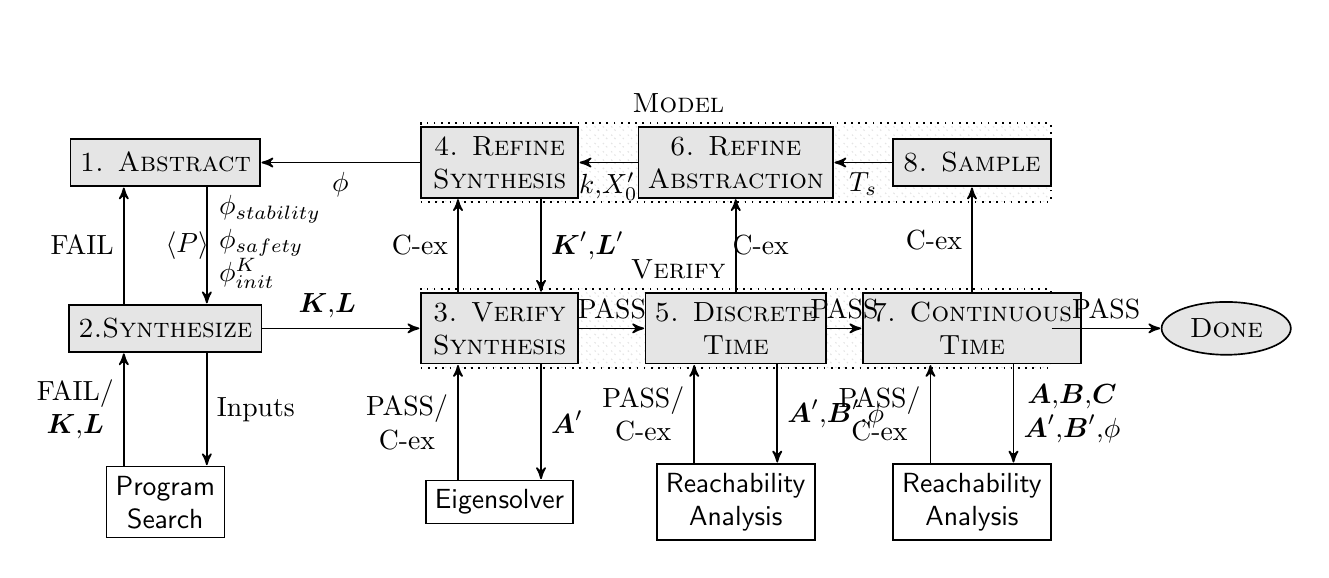
\begin{tikzpicture}[scale=0.3,->,>=stealth',shorten >=.2pt,auto, semithick, initial text=, ampersand replacement=\&,]
  \matrix[nodes={draw, fill=none, shape=rectangle, minimum height=.2cm, minimum width=.2cm, align=center}, row sep=.6cm, column sep=1cm] {
  \coordinate (aux1);\&\&
  \coordinate (aux2);
  \coordinate (aux3) at ([xshift=3cm]aux2); \\
  \node[minimum width=1.5cm, minimum height=0.6cm, fill=gray!20] (model1) {{\sc 1. Abstract}};
  \&\& complexnode/.pic={ 
     \node[rectangle,draw,dotted,
	minimum width=8cm,
	minimum height=1cm,
        pattern=north west lines, pattern color=gray!20,
	label={\sc Model~~~~~~~~~~~},] (model) {};
     \node[minimum width=2cm, minimum height=0.6cm, fill=gray!20] (model2) at ([xshift=-3cm]model.center) {{\sc 4. Refine}\\{\sc Synthesis}};
     \node[minimum width=2cm, minimum height=0.6cm, fill=gray!20] (model3) at ([xshift=0cm]model.center) {{\sc 6. Refine}\\{\sc Abstraction}};
     \node[minimum width=2cm, minimum height=0.6cm, fill=gray!20] (model4) at ([xshift=3cm]model.center) {{\sc 8. Sample}};
   } ;\\
   \node[minimum width=1.5cm, minimum height=0.6cm, fill=gray!20] (synth) {{\sc 2.Synthesize}};
   \&\&
   complexnode/.pic={ 
     \node[rectangle,draw,dotted,
	minimum width=8cm,
	minimum height=1cm,
        pattern=north west lines, pattern color=gray!20,
	label={\sc Verify~~~~~~~~~~~},] (verif) {};
     \node[minimum width=2cm, minimum height=0.6cm, fill=gray!20] (verif1) at ([xshift=-3cm]verif.center) {{\sc 3. Verify}\\{\sc Synthesis}};
     \node[minimum width=2cm, minimum height=0.6cm, fill=gray!20] (verif2) at ([xshift=0cm]verif.center) {{\sc 5. Discrete}\\{\sc Time}};
     \node[minimum width=2cm, minimum height=0.6cm, fill=gray!20] (verif3) at ([xshift=3cm]verif.center) {{\sc 7. Continuous}\\{\sc Time}};
   } 
   \& \node[ellipse, fill=gray!20] (done) {{\sc Done}};\\
   \& \\
   \node[minimum height=0cm] (gp) {{\sf Program}\\{\sf Search}};
   \&\&
   complexnode/.pic={ 
     \coordinate (aux);
   \node (bmc) at ([xshift=-3cm]aux.center) {\sf Eigensolver};
   \node (fp)  at ([xshift=0cm]aux.center) {\sf Reachability \\ \sf Analysis};
   \node (sv)  at ([xshift=3cm]aux.center) {\sf Reachability \\ \sf Analysis};
   }   
    \\
  };
   \path
    (synth.east) edge node[xshift=-0.5em,align=center] {$\mat{K}$,$\mat{L}$} (verif1.west)
    (verif1.east) edge node {PASS} (verif2.west)
    (verif2.north) edge node[xshift=.8cm] {C-ex} (model3.south)
    (verif2.east) edge node {PASS} (verif3.west)
    (verif3.north) edge node {C-ex} (model4.south)
    (model3.west) edge node {$k$,$X_0'$} (model2.east)
    (model4.west) edge node {$T_s$} (model3.east)
    ([xshift=-5em]fp.north) edge node[align=center]  {PASS/\\C-ex} ([xshift=-5em]verif2.south)
    ([xshift=-5em]sv.north) edge node[align=center]  {PASS/\\C-ex} ([xshift=-5em]verif3.south)
    ([xshift=5em]verif1.south) edge node[align=center] {$\mat{A}'$} ([xshift=5em]bmc.north)
    ([xshift=5em]verif2.south) edge node[align=center] {$\mat{A}'$,$\mat{B}'$,$\phi$} ([xshift=5em]fp.north)
    ([xshift=5em]verif3.south) edge node[align=center] {{$\mat{A}$,$\mat{B}$,$\mat{C}$}\\{$\mat{A}'$,$\mat{B}'$,$\phi$}} ([xshift=5em]sv.north)
    ([xshift=-5em]bmc.north) edge node[align=center]  {PASS/\\C-ex} ([xshift=-5em]verif1.south)
    (verif) edge node {PASS} (done)
    ([xshift=5em]synth.south) edge node[align=center] {Inputs} ([xshift=5em]gp.north)
    ([xshift=-5em]gp.north) edge node[align=center] {FAIL/\\$\mat{K}$,$\mat{L}$} ([xshift=-5em]synth.south)
    ([xshift=5em]model1.south) edge node[align=center,xshift=-.65cm] {$\langle P \rangle$} ([xshift=5em]synth.north) node[align=left,yshift=-0.7cm,xshift=.8cm] {{$\phi_{stability}$}\\{$\phi_{safety}$}\\ {$\phi_{init}^K$}}
   ([xshift=-5em]synth.north) edge node[align=center] {FAIL} ([xshift=-5em]model1.south);
   \path[->]
    ([xshift=-5em]verif1.north) edge node[align=center]  {C-ex} ([xshift=-5em]model2.south)
    ([xshift=5em]model2.south) edge node[align=center]  {$\mat{K}'$,$\mat{L}'$} ([xshift=5em]verif1.north)
    (model2.west) edge node[align=center] {$\phi$} (model1.east);

   %(verif4.north) edge node[align=center] {} ([xshift=10.5cm]aux2)
   %([xshift=10.5cm]aux2) edge node[align=center] {Increase Sampling Rate} (aux1);

 \end{tikzpicture}
}
\caption{CEGIS with Abstraction Refinement}
\label{fig:CEGARIS}
\end{figure*}

%-------------------------------
\section{Experimental Evaluation}
\label{exp:evaluation}
%-------------------------------

\jrronly{
%-------------------------------
\subsection{Description of the benchmarks}
\label{exp:benchmarks}
%-------------------------------
}
%\textcolor{red}{Iury: can you please describe the benchmarks?}

The benchmark suite employed to evaluate the proposed technique is 
composed by 18 MIMO models extracted from the literature~\cite{acrobot,cstr,CHEN1979389,KOKOTOVIC198023,gajic2008optimal,Franklin15,maglev,converters}.

In the verification module, we use the tool Axelerator~\cite{} .

\jrronly{
%%%%%%%%%%%%%%%%%%%%%%%%%%%%%%%%%%%%%%%%%%%%%%%%%%%%%%%%%%%%%%%%%%%%%%%%%%%%%%%%%%%%%%
\paragraph*{DC Motor}
%%%%%%%%%%%%%%%%%%%%%%%%%%%%%%%%%%%%%%%%%%%%%%%%%%%%%%%%%%%%%%%%%%%%%%%%%%%%%%%%%%%%%%

DC Motor benchmark describes the velocity dynamics of a basic 
brushed direct current electrical machine.

%%%%%%%%%%%%%%%%%%%%%%%%%%%%%%%%%%%%%%%%%%%%%%%%%%%%%%%%%%%%%%%%%%%%%%%%%%%%%%%%%%%%%%
\paragraph*{Automotive Cruise System}
%%%%%%%%%%%%%%%%%%%%%%%%%%%%%%%%%%%%%%%%%%%%%%%%%%%%%%%%%%%%%%%%%%%%%%%%%%%%%%%%%%%%%%

An automotive cruise control system is used to keep constant the speed 
of an automobile  tracking a desired speed reference, compensating 
disturbances and uncertainties related to relief and terrain.

%%%%%%%%%%%%%%%%%%%%%%%%%%%%%%%%%%%%%%%%%%%%%%%%%%%%%%%%%%%%%%%%%%%%%%%%%%%%%%%%%%%%%%
\paragraph*{Pendulum}
%%%%%%%%%%%%%%%%%%%%%%%%%%%%%%%%%%%%%%%%%%%%%%%%%%%%%%%%%%%%%%%%%%%%%%%%%%%%%%%%%%%%%%

A pendulum is system composed by a swinging point mass suspended from 
a frictionless pivot through a negligible mass rod.

%%%%%%%%%%%%%%%%%%%%%%%%%%%%%%%%%%%%%%%%%%%%%%%%%%%%%%%%%%%%%%%%%%%%%%%%%%%%%%%%%%%%%%
\paragraph*{Inverted Pendulum}
%%%%%%%%%%%%%%%%%%%%%%%%%%%%%%%%%%%%%%%%%%%%%%%%%%%%%%%%%%%%%%%%%%%%%%%%%%%%%%%%%%%%%%

An inverted pendulum is a system similar to the pendulum but the point 
mass must be equilibrated above the pivot point that is mounted on an 
one degree of freedom cart that moves over a track through a DC motor.

%%%%%%%%%%%%%%%%%%%%%%%%%%%%%%%%%%%%%%%%%%%%%%%%%%%%%%%%%%%%%%%%%%%%%%%%%%%%%%%%%%%%%%
\paragraph*{Magnetic Suspension}
%%%%%%%%%%%%%%%%%%%%%%%%%%%%%%%%%%%%%%%%%%%%%%%%%%%%%%%%%%%%%%%%%%%%%%%%%%%%%%%%%%%%%%

Magnetic suspension benchmark corresponds to the discrete model of a 
simple eletromagnet-ball system where a steel ball is levitated in air 
by the action of an electromagnetic force generated by an electromagnet.

%%%%%%%%%%%%%%%%%%%%%%%%%%%%%%%%%%%%%%%%%%%%%%%%%%%%%%%%%%%%%%%%%%%%%%%%%%%%%%%%%%%%%%
\paragraph*{Magnetic Pointer}
%%%%%%%%%%%%%%%%%%%%%%%%%%%%%%%%%%%%%%%%%%%%%%%%%%%%%%%%%%%%%%%%%%%%%%%%%%%%%%%%%%%%%%

Magnetic pointer is a pointer, that is usually employed in analogue 
gauges and indicators, whose angular position dynamics is controlled 
by a magnetic field.

%%%%%%%%%%%%%%%%%%%%%%%%%%%%%%%%%%%%%%%%%%%%%%%%%%%%%%%%%%%%%%%%%%%%%%%%%%%%%%%%%%%%%%
\paragraph*{1/4 Car Suspension}
%%%%%%%%%%%%%%%%%%%%%%%%%%%%%%%%%%%%%%%%%%%%%%%%%%%%%%%%%%%%%%%%%%%%%%%%%%%%%%%%%%%%%%

The 1/4 Car Suspension benchmark corresponds to the model of a single 
wheel suspension system of a car, {\it i.e.} the relative motion dynamics 
of a mass springer damp model that connects the car to one of its wheels.

%%%%%%%%%%%%%%%%%%%%%%%%%%%%%%%%%%%%%%%%%%%%%%%%%%%%%%%%%%%%%%%%%%%%%%%%%%%%%%%%%%%%%%
\paragraph*{Computer Tape Driver}
%%%%%%%%%%%%%%%%%%%%%%%%%%%%%%%%%%%%%%%%%%%%%%%%%%%%%%%%%%%%%%%%%%%%%%%%%%%%%%%%%%%%%%

Computer Tape Drive is a computer storage device used to read and write 
data on magnetic tapes.

%%%%%%%%%%%%%%%%%%%%%%%%%%%%%%%%%%%%%%%%%%%%%%%%%%%%%%%%%%%%%%%%%%%%%%%%%%%%%%%%%%%%%%
\paragraph*{Acrobot - Robot Manipulator}
%%%%%%%%%%%%%%%%%%%%%%%%%%%%%%%%%%%%%%%%%%%%%%%%%%%%%%%%%%%%%%%%%%%%%%%%%%%%%%%%%%%%%%

The Acrobot benchmark corresponds to the model of an two-link 
underactuated robot manipulator, linearized by partial 
feedback linearization~\cite{acrobot}.

%%%%%%%%%%%%%%%%%%%%%%%%%%%%%%%%%%%%%%%%%%%%%%%%%%%%%%%%%%%%%%%%%%%%%%%%%%%%%%%%%%%%%%
\paragraph*{High-order Systems from Chen et. al.}
%%%%%%%%%%%%%%%%%%%%%%%%%%%%%%%%%%%%%%%%%%%%%%%%%%%%%%%%%%%%%%%%%%%%%%%%%%%%%%%%%%%%%%

These benchmarks corresponds to a series of high-order system model 
generally used as example for order reduction techniques~\cite{CHEN1979389}.
 In this work, these benchmarks are used for evaluate the proposed control
 synthesis technique under critical conditions, {\it i.e.} with a greater 
 number of parameters to be considered.


%%%%%%%%%%%%%%%%%%%%%%%%%%%%%%%%%%%%%%%%%%%%%%%%%%%%%%%%%%%%%%%%%%%%%%%%%%%%%%%%%%%%%%
\paragraph*{Continuous Stirred Tank Reactor}
%%%%%%%%%%%%%%%%%%%%%%%%%%%%%%%%%%%%%%%%%%%%%%%%%%%%%%%%%%%%%%%%%%%%%%%%%%%%%%%%%%%%%%

This benchmark describes a linear model for PH dynamics of a PH 
neutralization process of an aqueous solution of sodium acetate with 
hydrochloric acid in a continuous flow stirred-tank reactor.

%%%%%%%%%%%%%%%%%%%%%%%%%%%%%%%%%%%%%%%%%%%%%%%%%%%%%%%%%%%%%%%%%%%%%%%%%%%%%%%%%%%%%%
\paragraph*{Flexible Beam}
%%%%%%%%%%%%%%%%%%%%%%%%%%%%%%%%%%%%%%%%%%%%%%%%%%%%%%%%%%%%%%%%%%%%%%%%%%%%%%%%%%%%%%

A Flexible Beam is a plant usually employed in vibration studies. It is 
composed by a flexible metallic structure with piezoceramic actuators 
and sensors.

%%%%%%%%%%%%%%%%%%%%%%%%%%%%%%%%%%%%%%%%%%%%%%%%%%%%%%%%%%%%%%%%%%%%%%%%%%%%%%%%%%%%%%
\paragraph*{Helicopter Longitudinal Motion}
%%%%%%%%%%%%%%%%%%%%%%%%%%%%%%%%%%%%%%%%%%%%%%%%%%%%%%%%%%%%%%%%%%%%%%%%%%%%%%%%%%%%%%

The Helicopter Longitudinal Motion benchmark describes the dynamics of 
transitional motion with respect to a longitudinal plane and the 
rotational motion around the longitudinal axis.

%%%%%%%%%%%%%%%%%%%%%%%%%%%%%%%%%%%%%%%%%%%%%%%%%%%%%%%%%%%%%%%%%%%%%%%%%%%%%%%%%%%%%%
\paragraph*{USCG cutter Tampa Heading Angle}
%%%%%%%%%%%%%%%%%%%%%%%%%%%%%%%%%%%%%%%%%%%%%%%%%%%%%%%%%%%%%%%%%%%%%%%%%%%%%%%%%%%%%%

The USCG cutter Tampa Heading Angle describes the heading angle 
dynamics of a Coast Guard cutter.

%%%%%%%%%%%%%%%%%%%%%%%%%%%%%%%%%%%%%%%%%%%%%%%%%%%%%%%%%%%%%%%%%%%%%%%%%%%%%%%%%%%%%%
\paragraph*{Voltage regulator}
%%%%%%%%%%%%%%%%%%%%%%%%%%%%%%%%%%%%%%%%%%%%%%%%%%%%%%%%%%%%%%%%%%%%%%%%%%%%%%%%%%%%%%

The voltage regulator benchmark~\cite{KOKOTOVIC198023} consists 
in a linear model of a synchronous machine connected to an 
infinite bus.
%%%%%%%%%%%%%%%%%%%%%%%%%%%%%%%%%%%%%%%%%%%%%%%%%%%%%%%%%%%%%%%%%%%%%%%%%%%%%%%%%%%%%%
\paragraph*{Guidance Control System}
%%%%%%%%%%%%%%%%%%%%%%%%%%%%%%%%%%%%%%%%%%%%%%%%%%%%%%%%%%%%%%%%%%%%%%%%%%%%%%%%%%%%%%

The Guidance Control System benchmark is another high-order system 
model used by Chen et al.~\cite{CHEN1979389}  in order reduction 
techniques. Guidance systems are used to determine the path of an 
autonomous vehicle movement.

%%%%%%%%%%%%%%%%%%%%%%%%%%%%%%%%%%%%%%%%%%%%%%%%%%%%%%%%%%%%%%%%%%%%%%%%%%%%%%%%%%%%%%
\paragraph*{Satellite Attitude Control System}
%%%%%%%%%%%%%%%%%%%%%%%%%%%%%%%%%%%%%%%%%%%%%%%%%%%%%%%%%%%%%%%%%%%%%%%%%%%%%%%%%%%%%%

This benchmark describes the dynamics of a satellite attitude, 
{\it i.e.} the orientation angles. An attitude control system must 
maintain the desired orientation of satellite with respect to an 
inertial frame during all the excursion. 

%%%%%%%%%%%%%%%%%%%%%%%%%%%%%%%%%%%%%%%%%%%%%%%%%%%%%%%%%%%%%%%%%%%%%%%%%%%%%%%%%%%%%%
\paragraph*{Springer-mass damper}
%%%%%%%%%%%%%%%%%%%%%%%%%%%%%%%%%%%%%%%%%%%%%%%%%%%%%%%%%%%%%%%%%%%%%%%%%%%%%%%%%%%%%%

The springer-mass damper systems are classic models for a lot of 
mechanical systems dynamics. This benchmark describes a mass that is 
fixed to a node through a springer and moves under the action of a 
input force, damping, and elastic force.

}

%-------------------------------
\subsection{Results}
\label{exp:results}
%-------------------------------
The technique was applied  to the benchmarks and the results can be seen in table \ref{tab:results}
\begin{table}
\centering
%
\begin{tabular}{| r | l | c | c | r | c | r |}
%
\hline
\# & \multicolumn{1}{|c|}{Benchmark} & \multicolumn{1}{|c|}{order}  & \multicolumn{1}{|c|}{$\mat{K}$} & \multicolumn{3}{|c|}{$\mat{K}+\mat{L}+T_s$} \\
   &                                  & & \multicolumn{1}{|c|}{Time} & \multicolumn{1}{|c|}{Min} & \multicolumn{1}{|c|}{Median} & \multicolumn{1}{|c|}{Max}\\\hline
1  & DC Motor          & 2 & 2.1\,s& 16,16  &   4.1\,s &   4.1\,s\\
2  & Helicopter        & 3  & 1.4\,s& 24,16  &   18.7\,s &   18.7\,s\\
3  & Inverted Pendulum & 4 &   0.6\,s& 16,24  &  308.4\,s &  308.4\,s\\
4  & Magnetic Pointer  & 2  & 44.1\,s& 24,16  &  7.7\,s &  7.7\,s \\
%5  & Magnetic Suspension & 2 & 0.6\,s& 16,24  &   0\,s &   0\,s\\
5  & Pendulum          & 2 & 14.0\,s& 16,16  &   3.4\,s &   3.4\,s\\
6  & Suspension        & 2 & 73.7\,s& 16,24  &   1316.2\,s &   1316.2\,s\\
7  & Tape Driver       & 3 & 68.3\,s& 16,24  &   57.8\,s &   57.8\,s\\
%9 & Satellite          & 2 &   0.7\,s& - &  - &  -\\ %unobservable
\hline
%
\end{tabular}
\vspace{0.05in}
\caption{Experimental results\label{tab:results}}
\end{table}

%%-------------------------------
%\subsection{Threats to validity}
%\label{exp:threats-to-validity}
%%-------------------------------
Since our synthesisers use abstract aproximations of the real dynamics, our solution is not complete.
it is possible to have models where a true solution is not found although it exists.
Soundness is ensured by the verifiers,but once again, since these use over-approximations of the real dynamics, they may also reject valid solutions, hence affecting completeness. 

%-------------------------------
\section{Conclusions}
\label{sec:conclusions}
%-------------------------------

\newpage
\bibliographystyle{splncs03}
\bibliography{paper}
\newpage
\appendix

%-------------------------------
\subsection{Overapproximating continuous time dynamics using discrete models}
\label{sec:cont_aa}
%-------------------------------
Our plant models derive from the discretization of
continuous time systems.  We therefore seek to establish a sound
overapproximation which does not only encompass the selected discretization,
but any chosen discretization in the time domain.

A dynamical system is a system in which a function describes the progression
of a state over time.  In a continuous domain with linear dynamics, it is
described by a first order Ordinary Differential Equation (ODE).
\begin{equation}
\dot{x}(t)=\mat{A}\vec{x}(t)+\mat{B}\vec{u}(t)% +\vec{w}(t)
\label{eq:dynamical}
\end{equation}

%where $\vec{w}$  is a continuous zero-mean white noise source with
%covariance $N ( 0 , Q )$ 
Furthermore, a control system may have a derived
output that is a linear combination of its states and inputs, which may
restricts the observability of the statespace from the output space.
\begin{equation}
\vec{y}(t)=\mat{C}\vec{x}(t)+\mat{D}\vec{u}(t)
\end{equation}

Discretization of a continuous dynamical system turns the ODE into a
difference equation, assuming zero-order hold for the input $\vec{u}$
%and continuous integration for the noise $\vec{w}$,
to
\begin{align}
\label{eq:discretization}
\vec{x}_{k+1} &= \mat{A}_d\vec{x}_k+\mat{B}_d\vec{u}_k\\% + \vec{w}_k\\
y_k &= \mat{C}_d \vec{x}_ k + \mat{D}_d \vec{u}_ k 
\end{align}
%with covariance for $\vec{w}_k$, $N ( 0 , Q_d )$
where
\begin{align}
\label{eq:discretize}
\mat{A}_d &= e^{\mat{A} T_s} = \mathcal{L}^{-1} { ( s \mat{I} - \mat{A} )^{-1} }_{t = T_s}\\
\mat{B}_d &= \int_{t = 0}^{T_s} e^{\mat{A} t} dt\ \mat{B} = \mat{A}^{-1} ( \mat{A}_d - \mat{I} ) \mat{B}\\
\mat{C}_d &= \mat{C}\\
\mat{D}_d &= \mat{D}
%\\Q_d &= \int_{t = 0}^{T_s} e^{\mat{A} t} Q e^{\mat{A}^T t} dt
\end{align}
and $T_s$ is the sample time. Then
\begin{align*}
\forall k, x(kT_s)=x_k \text{ and } y(kT_s) = y_k
\end{align*}

%+++++++++++++++++++++++++++++++++++++++++++++++++++++++++++++++++++++++++++++++
\section{Numerical representation and soundness} 
\label{sec:numeric_rep}
%+++++++++++++++++++++++++++++++++++++++++++++++++++++++++++++++++++++++++++++++

In embedded software programs interacting and/or simulating physical plants
it is of great importance to understand the effects of the chosen numeric 
representation for the continuous state-space and interacting discrete dynamics. 
\jrronly{
These representations are almost invariably approximations to the original
which are assumed to be precise enough as to not cause any trouble,
but it is precisely this assumption that often results in the most difficult and
dangerous errors.
There are generally speaking two formats for representing numbers in
programs. On one hand we have variable word length types which will
attempt to use as much memory as needed to precisely represent the
original domain (usually the reals). In this case the limitations are caused
by memory and speed, both of which are directly affected by the
increasingly larger word lengths. Multiple precision floating-point arithmetic
and software rationals are good examples of these cases. It is possible for
some of these data types to have memory constraints, at which point they
fall into the second category.
Fixed precision data types are most common in software programs.
}
Whether they be floating point or fixed point
\jrronly{ (of which integers are the special case for 0 decimal places) }
numbers, the problem arises in the misrepresentation of the reals%
\jrronly{ (or equivalent data type being represented) }.
Let $\mathbb{R}_{\langle M,F \rangle}$ be a fixed point domain with $M$ bits
representing the binary word length of the representation and $F$ bits
representing the prescaling $2^{-F}$ (\emph{i.e} the number of bits after
the decimal place).  We note that a negative $F$ denotes an integer
multiplication that adds $-F$ trailing zeros in the number represented by
$M$.
Let also $\mathbb{R}_{\langle M,[E] \rangle}$ be a floating point
domain with $M$ bits mantissa and $E$ bits exponent.  This domain
corresponds to $$\mathbb{R}_{\langle M,[E] \rangle} = \bigcup_F
\mathbb{R}_{\langle M,F \rangle} \mid F \in [2^{1-E}, 2^{E-1}]$$ This
definition important because it means that the distance between any two
numbers in the domain depends on the location of those numbers.  Since we
have shown that a floating point domain is a union of a number of fixed
point domains, we will continue our reasoning on fixed point only, which
will apply to the floating point domain by extension.  Operations on these
numbers will incur errors that can be bound
by~\cite{DBLP:conf/arith/BrainTRW15}.  We examine the most relevant ones:
%
\begin{enumerate}
\item Truncation\\
Let $\mathcal{F}_{\langle M,F \rangle} : \mathbb{R} \rightarrow \mathbb{R}_{\langle M,F \rangle}$
be a truncation function, defined as:
\begin{align*}
x_{\langle M,F \rangle}=\mathcal{F}_{\langle M,F \rangle}(x) = x-\delta \mid \delta=mod_F(x,c x_{\langle M,F \rangle})
\end{align*} 
where $mod_F(\cdot)$ is the modulus operation performed on the last bit of the representation ($2^{-F}$).\\
The number $\delta$ corresponds to the truncation error of the representation and it will propagate across operations.
\jrronly{
%
It is worth mentioning that not all systems truncate equally.  In the
definition above $\delta$ may be positive or negative, and even this
decision can be made dependent on the sign of $x$.  Common cases in computer
systems are: round downwards (\emph{ie} to $-\infty$), round upwards
(\emph{ie} to $+\infty$), and round to zero.  Rounding errors are cumulative
which means the overall error will statistically increase with every
operation, thus algorithms performing fewer operations can be more precise
in this respect than iterative ones.
%
}
\item Rounding\\
Every time an operation is performed on a number in the $\mathbb{R}_{\langle M,F \rangle}$ domain, an error may be
introduced due to truncation of the result. 
The following errors appear in simple operations:
\begin{enumerate}
\item Addition/Substraction
\begin{align*}
&x_{\langle M,F_1\rangle} \pm y_{\langle M,F_2\rangle}=z_{\langle M,F\rangle} + \delta,  F=\text{min}(F_1,F_2)\\
&\text{ where } |\delta| \leq 2^{-F} \text{ and } F_1=F_2 \Rightarrow \delta=0.
\end{align*}
\item Multiplication
\begin{align*}
&x_{\langle M,F_1\rangle} * y_{\langle M,F_2\rangle}=z_{\langle M,F\rangle} + \delta, \text{ where } F=F_1+F_2 \text{ and } |\delta| \leq 2^{-F}
\end{align*}
%\item Division\\
%The operations performed by our controllers in the FWL
%domain do not include division.  However, we do use division in computations
%at the precision of the plant.  Here the error depends on whether the
%divisor is greater or smaller than the dividend:  $x_{\langle M,F_1\rangle} / y_{\langle M,F_2 \rangle} = c_3 + \delta_{T3}$
%where $\delta_{T3}$ is $(\delta_{T2}\cdot x - \delta_{T1}\cdot y)/(\delta_{T2}^2 - \delta_{T2} y)$,
\end{enumerate}

\jrronly{
\item Overflow\\
Another source of error introduced by Finite Word Length representations is that of overflow.
The finite word length set a maximum representable number in the domain
$\pm \overline{M} \mid \overline{M}=2^{M-F}-2^{-F}$, which means that any number
outside this range cannot be accurately represented by the domain (\emph{eg} $\delta=x-\overline{M}$).
In the case of floating point, a special cases for infinity has been introduced, which addresses
some of these issues, but once the error has gone to infinity, the numbers become meaningless.
It is the responsibility of software designers and tools to account for overflows and either
supply saturation functions to prevent them or raise alarms in their presence. In the case
of verification, the latter is seen as a safety problem.
\item Null/Zeno behaviour\\
Whilst this work does not explore the effect of Zeno behaviours, it is worth noting that this
effect may also be caused by rounding errors in floating point programs. The reason for this
is that if an operation contains two numbers which belong to disjoint sub-domains
(\emph{ie} neither number can be represented in the domain of its counterpart), the
resulting operation may become a no-op/skip, subsequently destabilizing the program.
}
\end{enumerate}
We will use the domain $\mathbb{R}_{\langle C \rangle} \mid \langle C \rangle = \langle M_c,F_c \rangle$
to represent the fixed point precision of the controller, and 
$\mathbb{R}_{\langle P \rangle} \supseteq \mathbb{R}_{\langle C \rangle}$
to represent the domain of the plant model.
Thus any mathematical operations in our modelled digital controller will be executed in the
domain $\mathbb{R}_{\langle C \rangle}$, and all other calculations
in our model will be carried out in the domain $\mathbb{R}_{\langle
P \rangle}$.  The physical plant operates in the reals, which means
our verification phase must also account for the numerical error caused by representing the
physical plant at the finite precision $\mathbb{R}_{\langle P \rangle}$.

We will use these subindices to represent functions, number, vectors and matrices in their
corresponding domains. We further note that by choosing $\langle C \rangle = \langle M_c,[E_c] \rangle$
we extend the following to floating point reasoning.

%+++++++++++++++++++++++++++++++++++++++++++++++++++++++++++++++
\subsubsection{Quantization error}
\label{appendix:quantization}
%+++++++++++++++++++++++++++++++++++++++++++++++++++++++++++++++

Let $q_c=2^{-F_c},q_a=2^{-F_a},q_d=2^{-F_d}$ be the smallest difference
between two numbers in their corresponding domains.  Assuming that our
system truncates numbers to the nearest value, this means thet the error
$\delta$ introduced by the function $\mathcal{F}_{\langle * \rangle}$ is
$\delta_*=\mathcal{F}_{\langle * \rangle}(x)-x \in \left[-\frac{q_*}{2}\
\frac{q_*}{2}\right]$.  We note that in the case of floating point,the
choice of $F$ is taken from the largest multiplication found (e.g.,
$|\mat{A}|_1|\vec{x}|_\infty \mid \vec{x} \models \phi_\mathit{safety}$,
where $\phi_\mathit{safety}$ is defined in \ref{eq:safetyspec}). From these
equations we can define:
%
\begin{align*}
\nu_1 \in \left[-\frac{q_a}{2}\ \frac{q_a}{2}\right] \cap  \left[-\frac{q_c}{2}\ \frac{q_c}{2}\right],
\nu_2 \in \left[-\frac{q_d}{2}\ \frac{q_d}{2}\right]
\end{align*}

We may also bound $\nu_2'$ from \eqref{eq:uk} as follollows:
\begin{align*}
\delta\left(\mat{K}_{\langle C\rangle} \vec{x}_{\langle C\rangle} \right) &\in \left[ -p \frac{q_c}{2}\ \ p \frac{q_c}{2}\right]\\
{\vec{\nu_e}}_i &\in \left[ -(p+2) \frac{q_c}{2}\ \ (p+2) \frac{q_c}{2}\right], i \in [1, p]\\
\Rightarrow \nu_2' &\in \left[  -p(|\mat{K}_{\langle C \rangle}|_1+2) \frac{q_c}{2}\ \ p(|\mat{K}_{\langle C \rangle}|_1+2) \frac{q_c}{2}\right]
\end{align*}
Similarly we also find
\begin{align*}
\nu_1' &\in \left[  -p(|{\mat{C}_d}_{\langle C \rangle}|_1+2) \frac{q_c}{2}\ \ p(|{\mat{C}_d}_{\langle C \rangle}|_1+2) \frac{q_c}{2}\right]
\end{align*}
The proof derives from $|\mat{K}\vec{x}| \leq |\mat{K}|_1|\vec{x}|_\infty$.

%-------------------------------
\section{Stability} 
\label{appendix:stabspecification}
%-------------------------------

There are a number of algorithms that can be
used for stability analysis~\cite{daes20161,Bessa16}.

A discrete-time LTI system as \eqref{eq:closedloopss} is
asymptotically stable if all the roots of its characteristic
polynomial (i.e., the eigenvalues of the closed-loop matrix $A_d - B_d
K$) are inside the unity circle of the complex plane, i.e., their
absolute values are strictly less than one~\cite{astrom1997computer}
(this simple sufficient condition can be generalised, however this is
not necessary in our work).  In this paper, we express this stability
specification $\phi_\mathit{stability}$ in terms of a check known as
\emph{Jury's criterion}~\cite{fadali}: this is an easy algebraic
formula to select the entries of matrix $K$ so that the closed-loop
dynamics are shaped as desired.



Since the canonical forms used in this work use the coefficients of the
characteristic polynomial $S(z)$ as opposed to its roots (which are
extremely hard to calculate for a SAT solver), we choose Jury's
criterion~\cite{astrom1997computer} to check the stability in the
$z$-domain in view of its efficiency.

We~consider the following form for $S(z)$:
%
\begin{equation*}
S(z) = z^{p}+a_1z^{p-1}+\cdots+a_{p-1}z+a_p.
\end{equation*}

and build the matrix
$\mat{M} \in \mathbb{R}^{p \times p}$ from its coefficients such that:
%
\begin{align*}
\mat{M}_{1,j}&=a_j\\
\mat{M}_{i+1,j}&=\left\{
\begin{array}{ll}
0,&j>p'\\
\mat{M}_{i,j}-\mat{M}_{i,p'-j+1}\frac{\mat{M}_{i,1}}{\mat{M}_{i,p'}} &j\leq p'
\end{array}
\right.\\
p'&=p-i+1
\end{align*}
%
$S(z)$ is the characteristic polynomial of a stable system if and
only if the following conditions hold~\cite{astrom1997computer}:
\begin{align*}
\phi_\mathit{stability}(S) \equiv
(S(1) > 0) \wedge ((-1)^p S(-1) > 0) \wedge (|a_p| < 1) \wedge \bigwedge\limits_{i=1}^p (\mat{M}_{i,1} > 0).
\end{align*}


%-------------------------------
\section{Proofs of theorems}
%-------------------------------
\setcounter{theorem}{0}
\setcounter{corollary}{0}
 %+++++++++++++++++++++++++++++++++++++++++++++++++++++++++++++++++++++++++++++++
 \subsubsection{Discrete dynamics using reals for systems without inputs}\label{asec:real_discrete_no_inputs}
 %+++++++++++++++++++++++++++++++++++++++++++++++++++++++++++++++++++++++++++++++
 \begin{theorem}
 Given $\dot{\vec{x}}=\mat{A}\vec{x}$, where $\mat{A}=\mat{S}\mat{J}\mat{S}^{-1}$, the expression
 \begin{align}
 \vec{x}_T&=\vec{x}(t=T)=\mat{A}_{T}\vec{x}_0\\
 \mat{A}_{T}&= \mat{S}
 \left [ \begin{array}{cccc}
 e^{T\lambda_1}  & s_1\frac{T^{1}e^{T\lambda_i}}{(1)!} & \hdots  & s_i\frac{T^{p-1}e^{T\lambda_i}}{(p-i)!} \\
0 & e^{T\lambda_i}  & s_i\frac{T^{j-i}e^{T\lambda_i}}{(j-i)!} & \vdots \\
\vdots & & \ddots & \vdots \\
0 & \cdots & 0  &e^{T\lambda_i} \\
\end{array} \right ]
 \mat{S}^{-1}
 \label{eq:continuous_tube_dyn}\\
 &\text{where } s_i=\left\{\begin{array}{cc}1&gm(\lambda_i)>1\\0&gm(\lambda_i)=1\end{array}\right.,\nonumber
 \end{align}
$\lambda_i \in \mat{J}$ are the eigenvalues of $\mat{A}$, and $gm(\lambda_i)$ is the geometric multiplicity of $\lambda_i$.  $\vec{x}_T$ is a witness of the system $\dot{\vec{x}}(t)=\mat{A}\vec{x}$ at time t=T.
 \end{theorem}
 \begin{corollary}
 If $\mat{J}$ is diagonal and there exists a discrete dynamics matrix for a sampling time $T_d$ such that $A_d=e^{\mat{A} T_d}$, then $\vec{x}_k=A_d^k\vec{x} : k \in (0,\infty)$ is a witness of the system at time $t=kT_d$.
 \end{corollary}
 \begin{proof}
 Let us recall equation \ref{eq:discretize}. The discrete representation of the system dynamics discretised with sample time $T_1$ is ruled by the formula
 $\mat{A}_1 = e^{\mat{A} T_1}$. From matrix theory, we have 
\begin{align}
 e^{\mat{A}}&=\sum_{k=0}^\infty \frac{1}{k!}\mat{A}^k
\end{align} 
\begin{align} 
 e^{\mat{S}\mat{J}\mat{S}^{-1}}&=\sum_{k=0}^\infty \frac{1}{k!}\left(\mat{S}\mat{J}\mat{S}^{-1}\right)^k
 =\mat{S} \left (\sum_{k=0}^\infty \frac{1}{k!}\mat{J}^k\right) \mat{S}^{-1}\nonumber\\
 &=\mat{S}e^{\mat{J}}\mat{S}^{-1}
\end{align} 
\begin{equation}
\mat{A}=\mat{S}\mat{J}\mat{S}^{-1} \Rightarrow \vec{A}_1 = \mat{S}\mat{J}_1\mat{S}^{-1}= \mat{S}e^{\mat{J} T_1}\mat{S}^{-1}.
 \end{equation}
 
 Let $\mat{J}$ be a diagonal matrix, such that 
 $${\lambda_1}_i=e^{\lambda_i T_1}, \forall \lambda_i \in \mat{J}.$$
 Let us now take a different sample rate $T_2$, such that 
 $${\lambda_2}_i=e^{\lambda_i T_2}, \forall \lambda_i \in \mat{J}.$$
 We can then say that 
 \begin{equation}
 {\lambda_2}_i=e^{\lambda_i T_1 \frac{T_2}{T_1}}={\lambda_1}_i^{\frac{T_2}{T_1}} \Rightarrow A_2=A_1^{\frac{T_2}{T_1}}.
 \end{equation}
 This proves the theorem for $gm(\lambda_i)=1$.
 We now note that given an exponentiated Jordan form with geometric multiplicity, the upper diagonal terms can be
 referenced to the original eigenvalues modified by the sampling rate.
  Let $\mat{J}\in \mathbb{R}^{p \times p}$ be a Jordan Canonical matrix.
 Then
\begin{align}
 \mat{J}_1&=\sum_{k=0}^\infty \frac{1}{k!}\left(\mat{J}T_1\right)^k=\sum_{k=0}^\infty \frac{1}{k!} \left [ \begin{array}{cccc}
 \lambda_i^k  & \binom{k}{1}  \lambda^{k-1} & \hdots  & \binom{k}{p-1} \lambda_i^{k-p+1} \\
& \lambda_i^k  & \binom{k}{1}  \lambda_i^{k-1} & \vdots \\
\vdots & \ddots & \ddots & \vdots \\
& &  &\lambda_i^k \\
\end{array} \right ] T_1^k
\end{align}
The eigenvalues remain the same as in the diagonal case, but the upper triangular terms are of the form:
\begin{align}
\forall j>i, c_{ij}&=\sum_{k=j-i}^\infty \frac{1}{k!}\binom{k}{j-i} \lambda_i^{k-(j-i)}T_1^k\\
&=\frac{1}{(j-i)!}\sum_{k=j-i}^\infty \frac{1}{(k-(j-i))!} \lambda_i^{k-(j-i)}T_1^k\nonumber\\
&=\frac{T_1^{j-i}e^{\lambda_i T_1}}{(j-i)!}\nonumber
\end{align}
which completes the proof for $gm(\lambda_i)>1$.
\end{proof}

 %+++++++++++++++++++++++++++++++++++++++++++++++++++++++++++++++++++++++++++++++
 \subsubsection{Discrete dynamics using reals for systems with parametric inputs}\label{asec:real_discrete_param_inputs}
 %+++++++++++++++++++++++++++++++++++++++++++++++++++++++++++++++++++++++++++++++
\begin{theorem}
The expression
 \begin{align}
 \vec{x}_T&=\vec{x}(t=T)=\mat{A}^{-1}\vec{x}_T'\nonumber\\
\vec{x}_T'&=\mat{A}\mat{A}_T\vec{x}_0 + (\mat{I}-\mat{A}_T)\mat{B}\vec{u} : \forall t \leq T,\ \vec{u}(t)=\vec{u} 
 \end{align}
 with $\mat{A}_T$ as per \eqref{eq:continuous_tube_dyn} is a witness of the system $\dot{\vec{x}}(t)=\mat{A}\vec{x}(t)+\mat{B}\vec{u}(t)$ at time $T$ given a parametric input $\vec{u}$.
 \end{theorem}
 \begin{corollary}
 If $\mat{J}$ is diagonal and there exists a discrete dynamics matrix for a sampling time $T_d :  A_d=e^{\mat{A} T_d}$, then $\vec{x}_k=A_d^k\vec{x}+(\mat{I}-\mat{A}_d^k\mat{B}\vec{u}) : k \in (0,\infty)$ is a witness of the system at time $kT_d$.
 \end{corollary}
 \begin{proof}
 We begin by expanding the equation
 \begin{align}
 \vec{x}_T&=\mat{A}^{-1}\vec{x}_T'\nonumber\\
 &=\mat{A}_T\vec{x}_0 + \mat{A}^{-1}(\mat{I}-\mat{A}_T)\mat{B}\vec{u}\nonumber\\
 &= \mat{A}_T\vec{x}_0 + \mat{B}_T\vec{u}
 \end{align}
 where $\mat{A}_T=e^{\mat{A}T}$ and $\mat{B}_T=\mat{A}^{-1}(\mat{I}-\mat{A}_T)\mat{B}$ correspond to $\mat{A}_d$ and $\mat{B}_d$ in equation \eqref{eq:discretize}
 \end{proof}

 %+++++++++++++++++++++++++++++++++++++++++++++++++++++++++++++++++++++++++++++++
 \subsubsection{Discrete dynamics using reals for systems with discrete time feedback inputs}\label{asec:real_discrete_feedback_inputs}
 %+++++++++++++++++++++++++++++++++++++++++++++++++++++++++++++++++++++++++++++++

The final case we analyse here is that of hybrid time systems, where the
plant dynamics evolve in continuous time while the feedback dynamics evolve
in discrete time.

\begin{theorem}
The expression
 \begin{align}
 \vec{x}_{t} &= (\mat{A}_{t-kT_s}-\mat{B}_{t-kT_s}\mat{K}) (\mat{A}_d-\mat{B}_d\mat{K})^k\vec{x}_0
 \label{eq:cyber_feedback}
 \end{align}
 with $\mat{A}_t, \mat{B}_t$ as per \eqref{eq:continuous_tube_dyn} and $\mat{A}_d, \mat{B}_d$ as per equation \eqref{eq:discretize} is a witness of the system
 \begin{align}
 \dot{\vec{x}}_{t} &= \mat{A}\vec{x}+\mat{B}\vec{u}_t\nonumber\\
 \vec{u}_t&=\mat{K}\vec{x}_k  \mid  kT_s \leq t < (k+1)T_s
 \end{align}
 \end{theorem}

\begin{proof}
Let $\mat{K}$ be a feedback controller such that $\vec{u}_k=-\mat{K}\vec{x}_k$ at time $t=kT_s$. Let the output of
the feedback system be a zero order holder such that $\vec{u}(t+kT_s)=\vec{u}(kT_s) : 0 \leq t < T_s$.
The closed loop dynamics of the system between times $kT_s$ and $kT_s+T_s$ are
\begin{equation}
\vec{x}_{k,t}=\mat{A}_t\vec{x}_k-\mat{B}_t\mat{K}\vec{x}_k = (\mat{A}_t-\mat{B}_t\mat{K})\vec{x}_k : 0 \leq t < T_s
\end{equation}
We further explore the dynamics across discrete time boundaries. Let $\mat{A}_d=\mat{A}_{T_s}$ and $\mat{B}_d=\mat{B}_{T_s}$
\begin{align}
\vec{x}_{k}&=\vec{x}_{k-1,T_s}= (\mat{A}_d-\mat{B}_d\mat{K})\vec{x}_{k-1}\\
\vec{x}_{k,T_s} &= (\mat{A}_d-\mat{B}_d\mat{K}) (\mat{A}_d-\mat{B}_d\mat{K})\vec{x}_{k-1}
\end{align}
which accelerating results becomes
\begin{align}
\label{eq:feedback_sampled_cont}
\vec{x}_{k} &= (\mat{A}_d-\mat{B}_d\mat{K}) ^k\vec{x}_0\\
\vec{x}_{t} &= (\mat{A}_{t-kT_s}-\mat{B}_{t-kT_s}\mat{K}) (\mat{A}_d-\mat{B}_d\mat{K})^k\vec{x}_0
\label{eq:feedback_cont}
\end{align}
\end{proof}

%+++++++++++++++++++++++++++++++++++++++++++++++++++++++++++++++++++++++++++++++
\subsubsection{Time delay on discrete time feedback systems} \label{sec:delay}
%+++++++++++++++++++++++++++++++++++++++++++++++++++++++++++++++++++++++++++++++
\begin{theorem}
The error introduced by a delay $t_d$ in the control output $\vec{u}_k$ of a discrete feedback controller for a continuous LTI system can be modelled as a non-deterministic noise signal upperbound by 
\begin{align}
|{\vec{y}_e}_{k}|_1 \leq q_t, \text{ where } q_t=&(|\mat{C}(\mat{B}_{T_s}-\mat{B}_{t_s})|_1+|\mat{C}\mat{A}_{t_s}\mat{B}_{t_d}|_1)|U|_\infty
\end{align}
\end{theorem}

\begin{proof}
Let us look at equations \eqref{eq:feedback_sampled_cont} and
\eqref{eq:feedback_cont}.  When we introduce an arbitrary delay $T_d$ where
$t_d=T_d$ and $t_s=T_s-T_d$ we obtain:
%
\begin{align}
\vec{x}_{k} &=\mat{A}_{t_s}(\mat{A}_{t_d}\vec{x}_{k-1}-\mat{B}_{t_d}\mat{K}\vec{x}_{k-2})-\mat{B}\mat{K}\vec{x}_{k-1}\nonumber\\
&=  (\mat{A}_{T_s}-\mat{B}_{t_s}\mat{K})\vec{x}_{k-1}-\mat{A}_{t_s}\mat{B}_{t_d}\mat{K}\vec{x}_{k-2}
\label{eq:delay_cont}
\end{align}
%
Differentiating with the expected progression without delay, we get a delay
error:
%
\begin{align}
{\vec{x}_e}_{k}=&(\mat{B}_{T_s}-\mat{B}_{t_s})\mat{K}\vec{x}_{k-1}-\mat{A}_{t_s}\mat{B}_{t_d}\mat{K}\vec{x}_{k-2}\nonumber\\
=&(\mat{B}_{T_s}-\mat{B}_{t_s})\vec{u}_{k}-\mat{A}_{t_s}\mat{B}_{t_d}\vec{u}_{k-1}
\end{align}
Rather than explicitly calculate this error, we will find an upper bound. Let $|U|_\infty=max(|\vec{u}|_\infty \mid \vec{u} \in U)$ be the maximum infinity norm of a vector set, propagating the error to the output $\vec{y}_k$ we have:
\begin{align}
|{\vec{y}_e}_{k}|_1 \subseteq &(\mat{C}(\mat{B}_{T_s}-\mat{B}_{t_s})+\mat{C}\mat{A}_{t_s}\mat{B}_{t_d})U
\end{align}
\end{proof}
We overapproximate the effects of this vector by introducing a noise signal at the output $\nu_t=[-q_t\ q_t]$ and use the dynamics of the system without delay.

%-------------------------------
\subsection{Transient response} 
\label{asec:transientspecification}
%-------------------------------

\begin{theorem}
Given a set of eigenvalues for a discrete time model of an $n^{th}$ order system $\lambda_i =e^{\omega_i}: i \in [1\ n]$, the settling time of the system is upperbounded by
\begin{equation}
t_s<-log_{|\overline{\lambda}|}({p_s}) : |\overline{\lambda}| =\max(|\lambda_i|) \wedge |\overline{\lambda}|<1,\ \forall i \in [1\ n]
\label{eq:set_time}
\end{equation}
where $0\leq p_s \leq 1$ is the desired percentage of the target within to remain after $t_s$.
\end{theorem} 
\begin{proof}
In a SISO system, there are two values that typically define the
response-time of the system (using a step response).
%
\begin{enumerate}
\item The \emph{rise time} is defined as the time it takes the output to reach a percentage (eg $90\%$) of the target value given a step chnage in the input.
\item The \emph{settling time} is defined as the time it takes the output to stabilize within a margin of the target value (eg $10\%$).
\end{enumerate} 
%
In the case of first and second order systems, the decay is governed by the equations 
%
\begin{align*}
&y_{decay}=
&\left\{
\begin{array}{cc}
e^{-|\omega| t}& 1^{st} order\\
e^{\zeta |\omega| t}\left(\frac{\sin\left(|\omega| t\sqrt{1-\zeta^2}+\sin^{-1}\sqrt{1-\zeta^2}\right)}{\sqrt{1-\zeta^2}} \right)&\zeta<1\\
e^{-|\omega| t}-|\omega| t e^{-|\omega| t}&\zeta=1\\
\frac{|\omega| e^{-|\omega_2| t}-|\omega_2| e^{-|\omega| t}}{|\omega|-|\omega_2|}&\zeta>1\end{array}\right.
\end{align*}
where $|\omega|$ and $|\omega_2|$ are the magnitudes of the eigenvalues (roots) of the system and  $\zeta=-\cos(\theta)$ where $\theta$ is the polar angle of the conjugate pair if it exists ($\zeta \geq 1$ if it doesn't).
These equations become increasingly complicated for higher order systems. However, we note their strong dependency on the magnitude of the eigenvalues, and use this property to define an upperbound on the decay function.
All of the above equations will decay faster than $e^{-|\omega| t}$ given $|\omega| < |\omega_2|$, hence we may use this function as our upper bound.

Given a closed loop single output LTI system of order $n$ with dynamics
\begin{equation}
\left\{\begin{array}{c}\vec{x}_k=\mat{A}\vec{x}_{k-1}\\ \vec{y}_k=\mat{C}\vec{x}_k\end{array}\right. \Rightarrow \left\{ \begin{array}{c}\vec{x}_k'=\mat{J}\vec{x}_{k-1}'\\ \vec{y}_k=\mat{C}\mat{S}\vec{x}_k'\end{array}\right. : \left\{ \begin{array}{c}\mat{A}=\mat{S}\mat{J}\mat{S}^{-1} \\ \vec{x}_k'=\mat{S}^{-1}\vec{x}_k\end{array}\right.
\label{eq:eigendynamics}
\end{equation}
%
the output decay is a linear combination of the decay of eigenvalues or
eigenvalue pairs.  Let $\mat{C}'\in \mathbb{R}^{1 \times n}=\mat{C}\mat{S}$. 
Since $\mat{C}'$ is constant, the output $y_k$ is a linear combination of
the states $\vec{x}'_k$.  We accelerate equation \eqref{eq:eigendynamics} to
obtain
%
\begin{align}
%\vec{x}_k'&=\mat{J}^k\vec{x}_0' \\
y_k&=\mat{C}'\mat{J}^k\vec{x}_0 = \sum_{i=0}^p \left( c_i \lambda_i^k + c_{il}\binom{k}{l} \lambda_i^{k-l}\right)\\
|y_k|&\leq \sum_{i=0}^n \left|c_i + c_{il}\binom{k}{l} \lambda_i^{-l}\right||\lambda_i^k|
\end{align}
%
where the second  part of the equation corresponds to the upper diagonal
terms of the Jordan blocks.  We also have $|\lambda_i^k|\leq
|\overline{\omega}^k|$,hence
%
\begin{align}
|y_k|&\leq |\overline{\omega}^k|\sum_{i=0}^n \left|c_i + c_{il}\binom{k}{l} \lambda_i^{-l}\right|
\end{align}
%
Since we are synthesising the eigenvalues, rather than solve this formula
for complex Jordan Shapes, we will restrict our synthesiser to provide
solutions with distinct eigenvalues (which is by far the most common case). 
Therefore the right hand terms dissappear and we obtain
%
\begin{align}
|y_k|&\leq |\overline{\omega}^k|\sum_{i=0}^n |c_i|
\end{align}

Hence the overall decay of the system is always smaller
than $d=e^{-|\overline{\omega}| t}$ where $0\leq d\leq 1$ is the remaining
percentage of the decay expressed.  Reversing we have
$t=-\frac{ln(d)}{|\overline{\omega}|}=-\frac{ln(d)}{ln(|\overline{\lambda}|)}$. 
replacing for $p_s$ , $t_s$, and $\overline{\lambda}$ we get equation
\eqref{eq:set_time}
%
\qed
\end{proof}


%%-------------------------------
%\section{Stability of Closed-loop Models}
%\label{sec:appendix-stability}
%%-------------------------------
%
%%-------------------------------
%\subsection{Stability of closed-loop models with fixed-point controller error}
%\label{sec:stab_FWL}
%%-------------------------------
%
%The proof of Jury's criterion~\cite{fadali} relies on the fact that the relationship between states and
%next states is defined by $x_{k+1} = (A_d - B_dK) x_k$, all computed
%at infinite precision.  When we employ a FWL digital controller, the
%operation becomes:
%%
%\begin{align*}
%x_{k+1} &= A_d \cdot x_{k} -(\mathcal{F}_{\langle I_c,F_c \rangle}(K)\cdot\mathcal{F}_{\langle I_c,F_c \rangle}(x_{k})).  \\
%x_{k+1} &= (A_d  - B_dK) \cdot x_k + B_dK\delta, 
%\end{align*}
%%
%where $\delta$ is the maximum error that can be introduced by the FWL
%controller in one step, i.e., by reading the states values once and
%multiplying by $K$ once.  We derive the closed form expression for $x_n$ as
%follows:
%%
%\begin{align*}
%x_{1} &= (A_d  - B_dK)x_0 + B_dK\delta \\
%x_{2} 
% &=(A_d  - B_dK)^2x_0 + (A_d  - B_dK)B_dK\delta + B_dK\delta \\
%x_{n} &= (A_d  - B_dK)^nx_0 + (A_d  - B_dK)^{n-1}B_dK\delta + ... \\  \nonumber & + (A_d  - B_dK)^1B_dK \delta + B_dK\delta \\
%  &= (A_d - B_dK)^nx_0 + \sum_{i=0}^{i=n-1}(A_d - B_dK)^iB_dk\delta. 
%\end{align*}
%
%The definition of asymptotic stability is that the system converges to a
%reference signal, in this case we use no reference signal so an
%asymptotically stable system will converge to the origin.  We know that the
%original system with an infinite-precision controller is stable, because we
%have synthesized it to meet Jury's criterion.  Hence, $(A_d - B_dK)^n x_0$ 
%must converge to zero.
%
%The power series of matrices
%converges~\cite{horn1990matrix} iff the eigenvalues of the matrix are less
%than~1 as follows:
%%
%%\begin{align*}
%$\sum_{i=0}^{\infty}T^i  = (I - T)^{-1}$, 
%%\end{align*}
%%
%where $I$ is the identity matrix and $T$ is a square matrix. Thus, our system will converge to the value 
%%
%\begin{align*}
%0 + (I - A_d + B_dK)^{-1}B_dk\delta \,. 
%\end{align*}
%%
%As a result, if the value $(I - A_d + B_dK)^{-1}B_dk\delta$ is within the
%safe space, then the synthesized fixed-point controller results in a safe
%closed-loop model.  The convergence to a finite value, however, will not
%make it asymptomatically stable.
%

\end{document}
